\subsection*{Tuần 6}

\subsubsection*{6.1 Mô tả công việc}

Trong tuần 6 của kỳ thực tập, sinh viên xây dựng chức năng thu nhận, xử lý và lưu trữ dữ liệu từ máy lọc nước, đồng thời phát triển dashboard hỗ trợ giám sát telemetry theo thời gian thực. Dữ liệu đầu vào được ESP32 publish lên HiveMQ Cloud theo cấu trúc đã chuẩn hóa trong tuần 5.

Các công việc chính gồm:

\begin{itemize}
    \item Cấu hình Device Monitor kết nối HiveMQ bằng MQTT over WebSocket.
    \item Subscribe topic \texttt{devices/telemetry}.
    \item Xây dựng API tiếp nhận bản tin từ MQTT Client.
    \item Parse và kiểm tra payload JSON.
    \item Chuẩn hóa \texttt{mcu\_id}, \texttt{tds}, \texttt{alert} và bổ sung \texttt{timestamp}.
    \item Lưu telemetry vào MySQL \texttt{smartwater\_database} qua schema migration dùng chung.
    \item Xây dựng danh sách MCU, bảng telemetry theo MCU và biểu đồ TDS theo thời gian.
    \item Kiểm tra luồng dữ liệu từ ESP32 đến giao diện giám sát.
\end{itemize}

\subsubsection*{6.2 Nội dung thực hiện}

\subsubsubsection*{6.2.1 Kiến trúc thu nhận telemetry}

Device Monitor là thành phần trung gian giữa HiveMQ và cơ sở dữ liệu. MQTT Client chạy trên trình duyệt thiết lập kết nối bảo mật đến HiveMQ Cloud, đăng ký topic và nhận bản tin ngay khi Broker chuyển tiếp dữ liệu.

Luồng dữ liệu được tổ chức như sau:

\begin{center}
ESP32 $\rightarrow$ HiveMQ $\rightarrow$ MQTT WebSocket Client $\rightarrow$ API Device Monitor
$\rightarrow$ Telemetry Service $\rightarrow$ Repository $\rightarrow$ MySQL
\end{center}

Việc tách các bước tiếp nhận, chuẩn hóa và lưu trữ giúp mỗi thành phần có một trách nhiệm rõ ràng, đồng thời thuận tiện cho việc kiểm tra lỗi tại từng giai đoạn.

Hình \ref{fig:week6-hivemq-architecture} minh họa vai trò của HiveMQ Broker trong mô hình truyền dữ liệu giữa thiết bị và các ứng dụng xử lý.

\begin{figure}[H]
    \centering
    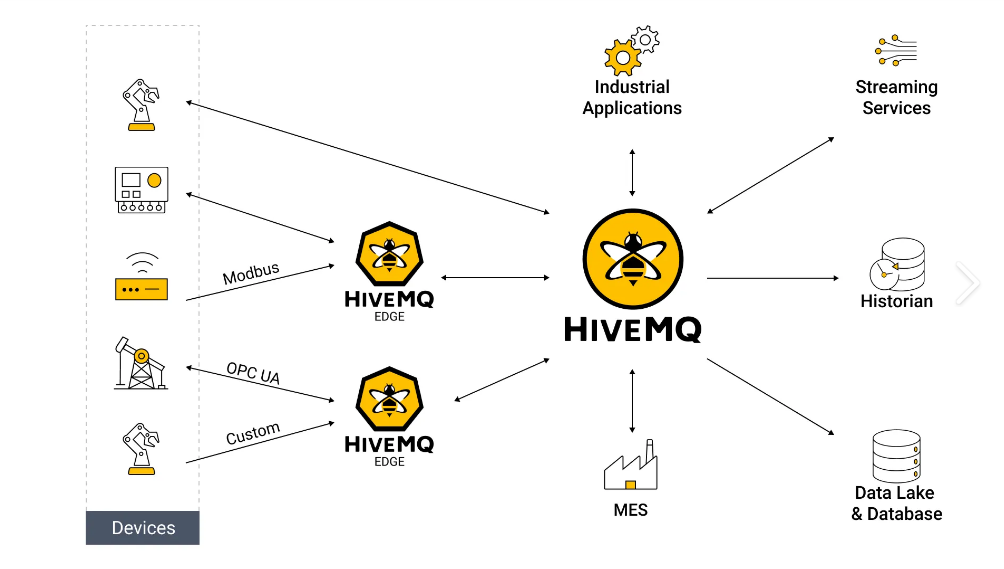
\includegraphics[width=0.90\linewidth]{include/image/hivemq.png}
    \caption{Vai trò của HiveMQ trong kiến trúc truyền dữ liệu IoT}
    \label{fig:week6-hivemq-architecture}
\end{figure}

\subsubsubsection*{6.2.2 Kết nối và subscribe HiveMQ}

Trang cấu hình Device Monitor cho phép khai báo địa chỉ Broker, cổng WebSocket, tài khoản và danh sách topic cần theo dõi. Cấu hình được lưu tại trình duyệt để phục vụ quá trình thử nghiệm.

Khi người dùng thực hiện kết nối, MQTT Client tạo địa chỉ WebSocket bảo mật có dạng:

\begin{verbatim}
wss://<broker>:<port>/mqtt
\end{verbatim}

Sau khi kết nối thành công, Client subscribe topic \texttt{devices/telemetry}. Sự kiện \texttt{message} được kích hoạt khi có telemetry mới; payload được chuyển thành chuỗi, parse JSON và gửi đến API của Device Monitor.

Các hình dưới đây ghi nhận cấu hình HiveMQ Cloud đã sử dụng trong quá trình thử nghiệm: cluster đang chạy, thông tin kết nối MQTT/TLS và quyền publish/subscribe của credential. Giá trị bí mật không được hiển thị trong báo cáo.

\begin{figure}[H]
    \centering
    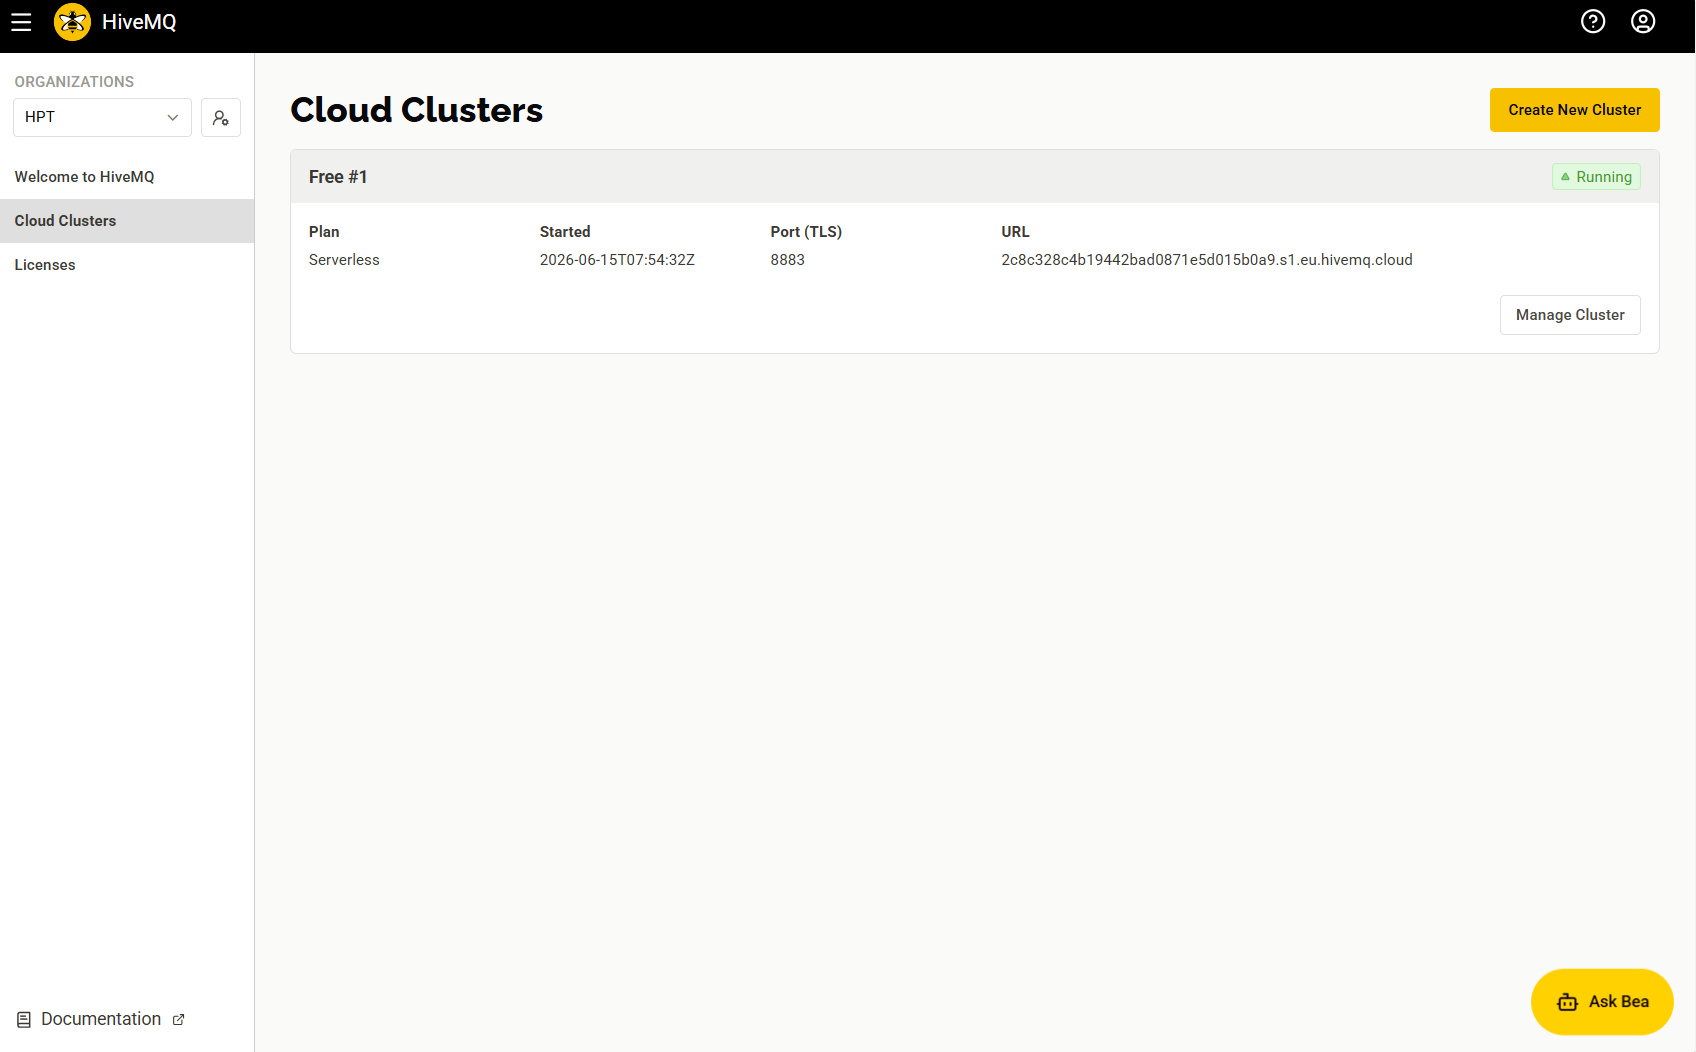
\includegraphics[width=0.95\linewidth]{include/web-UI/hivemq-cluster.png}
    \caption{HiveMQ Cloud cluster được cấu hình cho thử nghiệm}
    \label{fig:week6-hivemq-cluster}
\end{figure}

\begin{figure}[H]
    \centering
    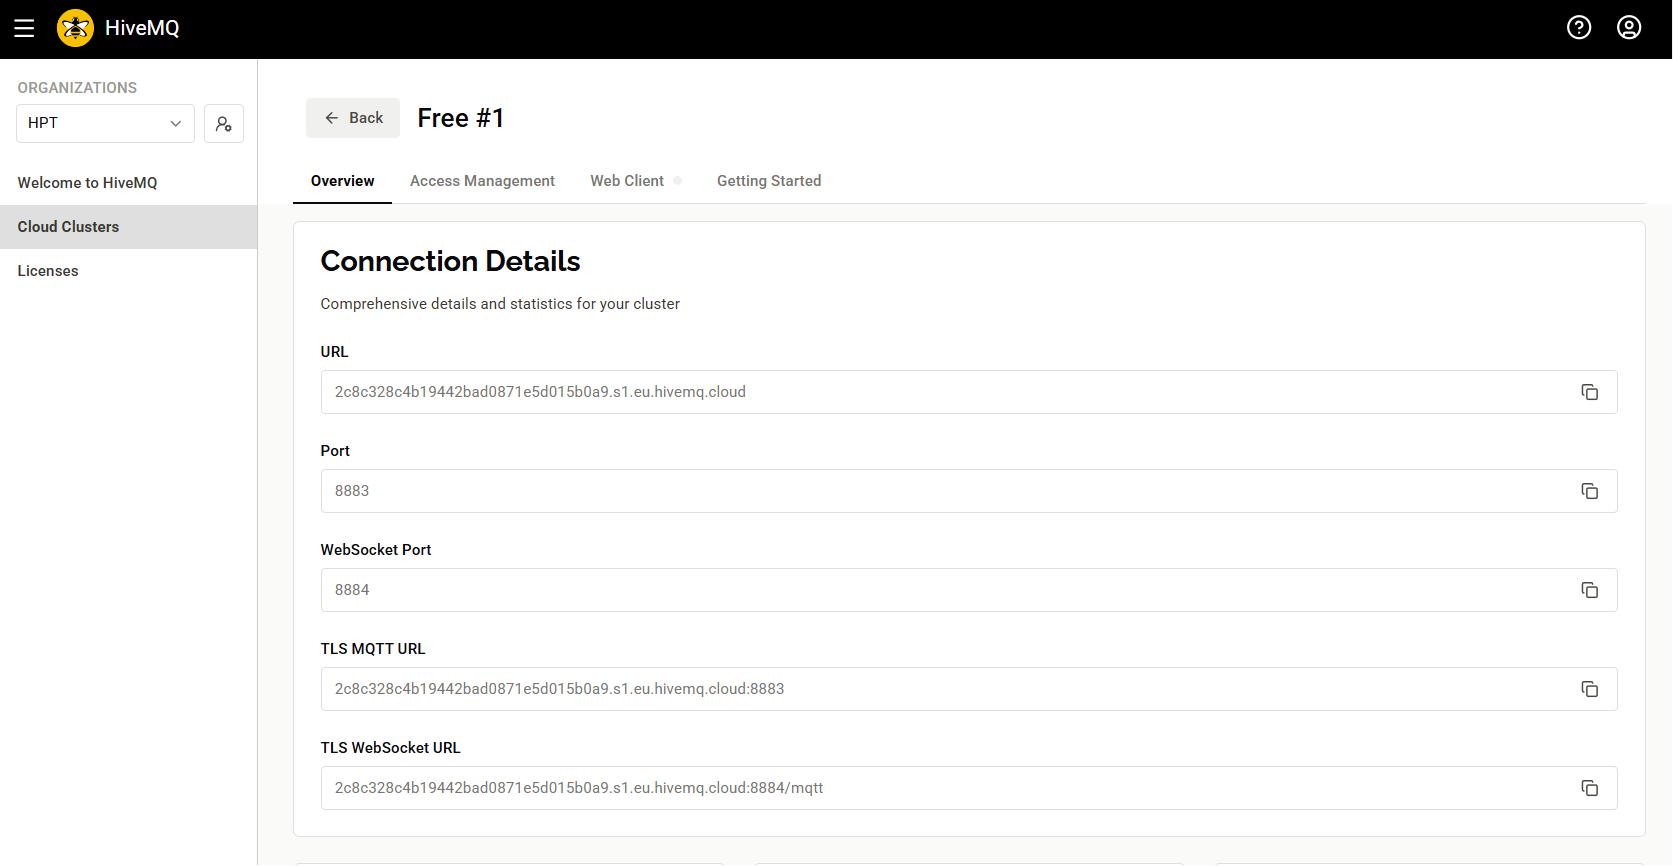
\includegraphics[width=0.95\linewidth]{include/web-UI/hivemq-connection.png}
    \caption{Thông tin kết nối MQTT TLS và WebSocket của HiveMQ Cloud}
    \label{fig:week6-hivemq-connection}
\end{figure}

\begin{figure}[H]
    \centering
    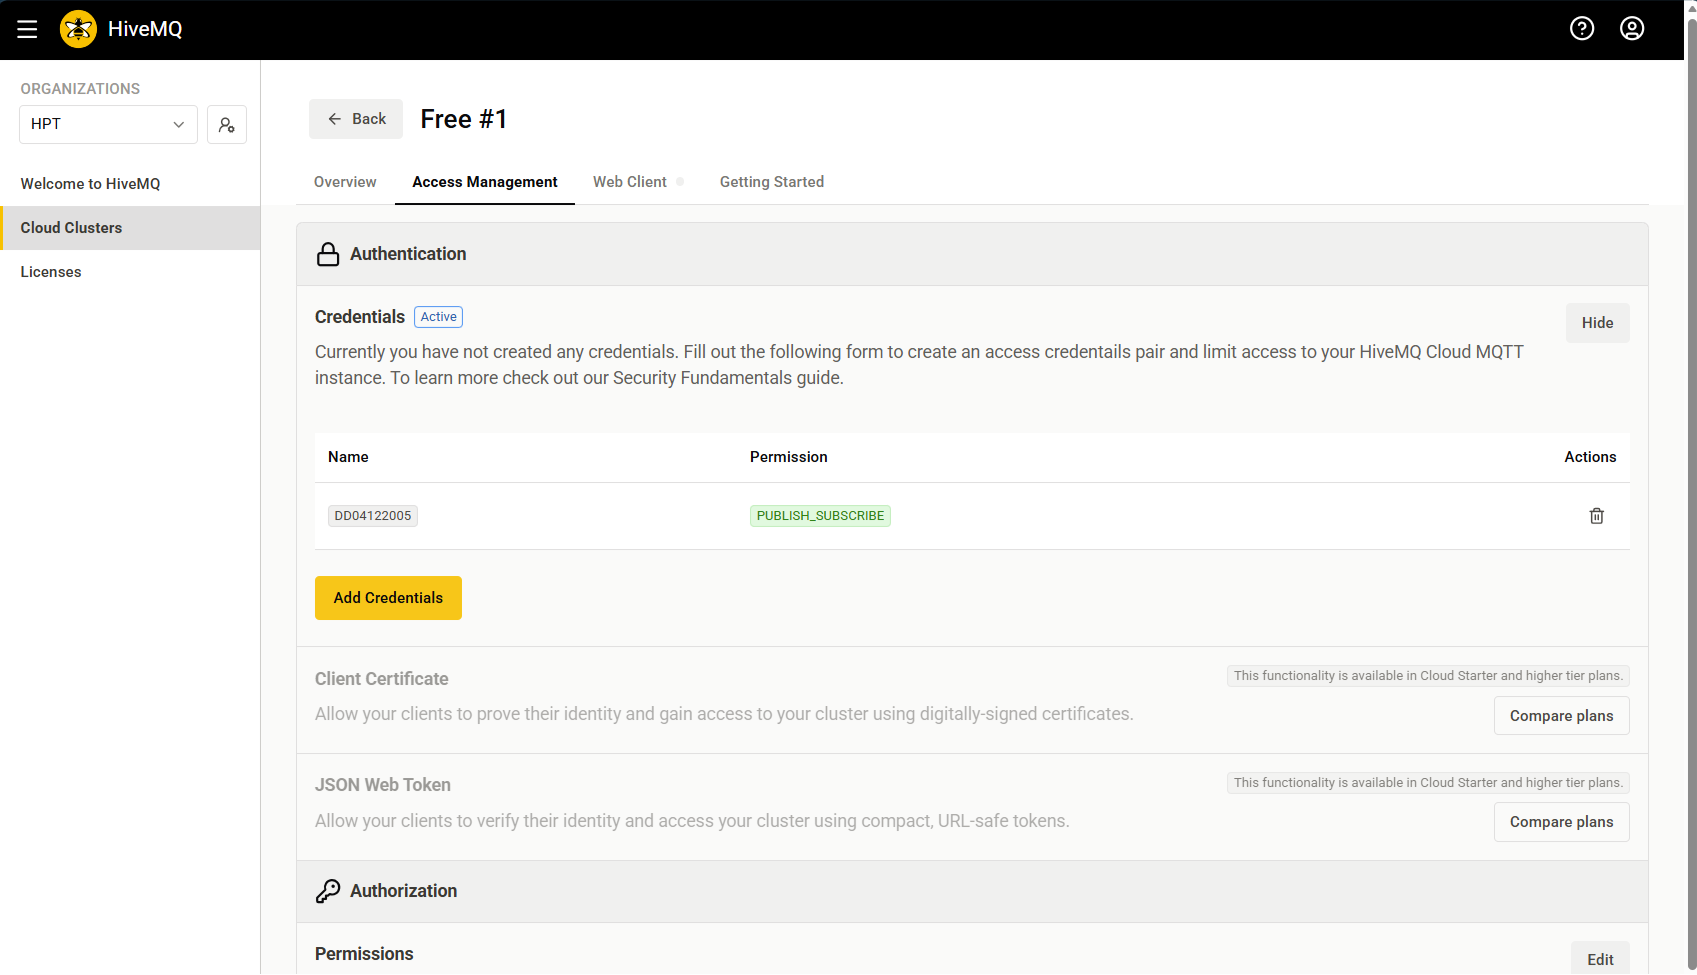
\includegraphics[width=0.95\linewidth]{include/web-UI/hivemq-credential.png}
    \caption{Credential HiveMQ Cloud với quyền publish và subscribe}
    \label{fig:week6-hivemq-credential}
\end{figure}

Web Client của HiveMQ được dùng để kiểm tra kết nối và subscription độc lập với Device Monitor. Hình \ref{fig:week6-hivemq-topic} minh họa khu vực đăng ký topic; Hình \ref{fig:week6-hivemq-webclient} cho thấy Web Client ở trạng thái kết nối.

\begin{figure}[H]
    \centering
    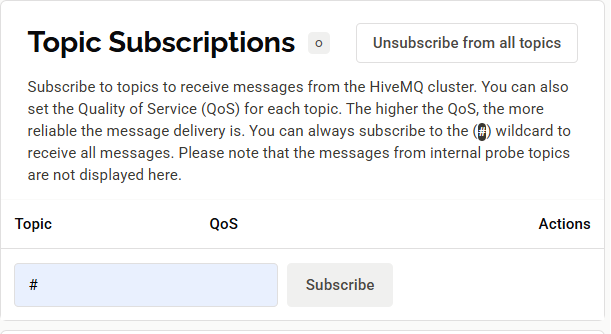
\includegraphics[width=0.70\linewidth]{include/web-UI/hivemq-sub-topic.png}
    \caption{Đăng ký topic trong HiveMQ Web Client}
    \label{fig:week6-hivemq-topic}
\end{figure}

\begin{figure}[H]
    \centering
    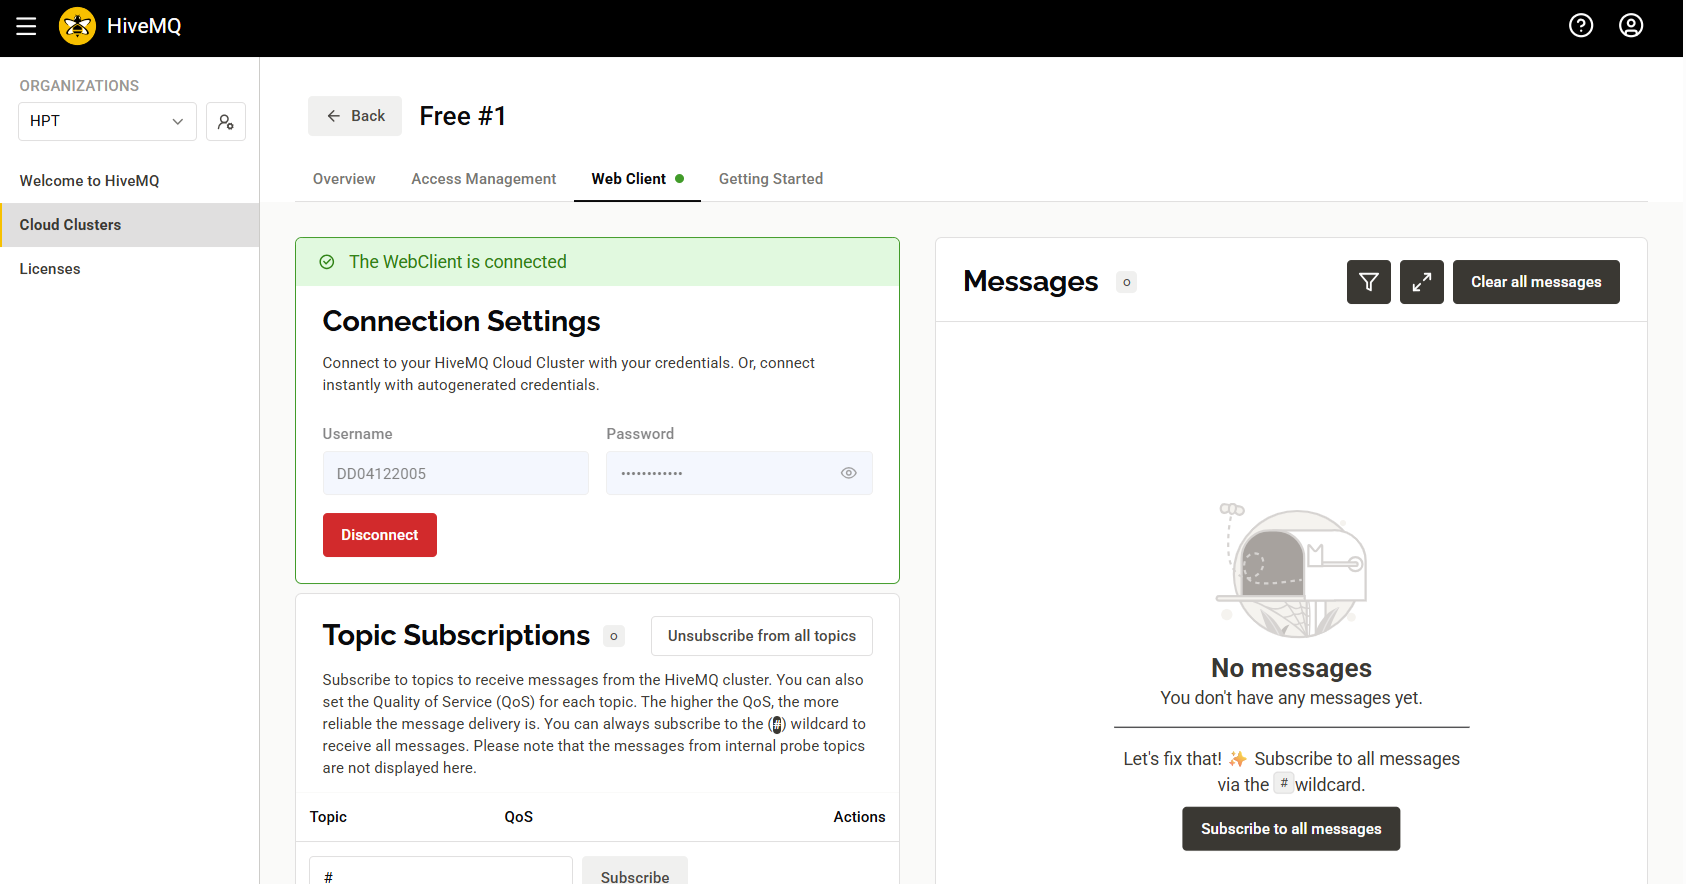
\includegraphics[width=0.95\linewidth]{include/web-UI/hivemq-webclient.png}
    \caption{HiveMQ Web Client ở trạng thái kết nối}
    \label{fig:week6-hivemq-webclient}
\end{figure}

\subsubsubsection*{6.2.3 Tiếp nhận và kiểm tra dữ liệu}

API telemetry tiếp nhận ba thành phần gồm topic, payload và nguồn dữ liệu. Telemetry Service thực hiện giải mã payload, làm phẳng các cấu trúc JSON lồng nhau và lấy các trường cần thiết.

Dữ liệu sau chuẩn hóa có dạng:

\begin{verbatim}
{
  "topic": "devices/telemetry",
  "timestamp": "2026-07-26 10:30:00",
  "mcu_id": "ESP32_001",
  "tds": 185,
  "alert": "normal"
}
\end{verbatim}

Các quy tắc xử lý gồm:

\begin{itemize}
    \item \texttt{mcu\_id} là trường bắt buộc, được chuẩn hóa thành chuỗi không rỗng tối đa 50 ký tự.
    \item \texttt{tds} được chuyển sang dữ liệu số nếu giá trị hợp lệ.
    \item \texttt{alert} là trường tùy chọn và được chuẩn hóa thành chuỗi khi payload có giá trị.
    \item \texttt{timestamp} được sinh tại Device Monitor theo thời điểm nhận bản tin.
    \item Bản tin thiếu hoặc sai \texttt{mcu\_id} bị từ chối trước khi ghi database.
\end{itemize}

\subsubsubsection*{6.2.4 Lưu telemetry vào MySQL}

Telemetry Repository sử dụng câu lệnh được chuẩn bị trước để ghi dữ liệu vào bảng \texttt{telemetry}. Schema được sở hữu bởi \texttt{smartwater-database}; Device Monitor chỉ kiểm tra bảng đã được migrate trước khi khởi động. Bảng gồm các trường chính:

\begin{itemize}
    \item \texttt{id}: khóa chính tự tăng.
    \item \texttt{timestamp}: thời điểm Device Monitor nhận dữ liệu.
    \item \texttt{topic}: topic MQTT nguồn.
    \item \texttt{mcu\_id}: định danh MCU dạng chuỗi, tối đa 50 ký tự.
    \item \texttt{tds}: giá trị TDS.
    \item \texttt{alert}: trạng thái cảnh báo.
\end{itemize}

Migration tạo index cho \texttt{timestamp}, \texttt{mcu\_id} và chỉ mục kết hợp \texttt{(mcu\_id, timestamp)} để hỗ trợ truy xuất lịch sử TDS theo từng MCU và theo thời gian. Bảng telemetry không khai báo khóa ngoại đến MCU, vì vậy dữ liệu telemetry được liên kết logic bằng \texttt{mcu\_id}. Device Monitor và SmartWater Admin cùng sử dụng MySQL \texttt{smartwater\_database}, nhờ đó dữ liệu giám sát và dữ liệu nghiệp vụ dùng cùng một nguồn schema.

\subsubsubsection*{6.2.5 Liên kết telemetry với dữ liệu nghiệp vụ}

Telemetry không liên kết trực tiếp với Customer hoặc Device bằng khóa ngoại, mà dùng \texttt{mcu\_id} làm định danh logic. Bảng \texttt{devices} gắn MCU bằng khóa ngoại \texttt{devices.mcu\_id -> mcus.mcu\_id}; SmartWater Admin truy xuất dữ liệu theo chuỗi quan hệ:

\begin{center}
Customer $\rightarrow$ Contract $\rightarrow$ Product $\rightarrow$ Device + MCU
$\rightarrow$ Telemetry
\end{center}

Mỗi Product thuộc tối đa một Contract tại một thời điểm. Device và MCU cùng được gắn vào Product; vì vậy telemetry của MCU có thể được xác định đúng máy lọc nước, hợp đồng và khách hàng đang sử dụng.

\subsubsubsection*{6.2.6 Xây dựng dashboard giám sát}

Dashboard Device Monitor cung cấp các thông tin tổng hợp:

\begin{itemize}
    \item Tổng số bản ghi telemetry.
    \item Số topic khác nhau.
    \item Số MCU đã gửi dữ liệu.
    \item Thời điểm của bản ghi mới nhất.
    \item Thống kê số lượng theo từng trạng thái cảnh báo.
\end{itemize}

Trang Telemetry Live được bố trí thành hai cột. Cột trái lấy các \texttt{mcu\_id} không trùng từ telemetry và hiển thị số bản ghi, thời điểm gần nhất. Khi chọn một MCU, cột phải tải bảng telemetry đã lọc và chuỗi TDS theo thời gian để vẽ biểu đồ.

Bảng telemetry gồm năm cột:

\begin{center}
\texttt{timestamp}, \texttt{topic}, \texttt{mcu\_id}, \texttt{tds}, \texttt{alert}
\end{center}

API đọc gồm \path|/api/mcus|, \path|/api/telemetry?mcu_id=...| và \path|/api/telemetry/chart?mcu_id=...|. Khi MQTT Client nhận bản tin mới và API lưu thành công, giao diện tải lại danh sách telemetry của MCU đang chọn. Nhờ đó người quản trị có thể theo dõi dữ liệu mới mà không cần thao tác trực tiếp với Broker hoặc cơ sở dữ liệu.

\subsubsubsection*{6.2.7 Xử lý lỗi}

Trong quá trình phát triển, sinh viên bổ sung cơ chế xử lý lỗi tại các điểm chính:

\begin{itemize}
    \item Hiển thị trạng thái khi thiếu cấu hình Broker.
    \item Thông báo lỗi kết nối hoặc ngắt kết nối MQTT.
    \item Từ chối payload không phải JSON hợp lệ hoặc thiếu \texttt{mcu\_id}.
    \item Trả HTTP 422 cho dữ liệu đầu vào không hợp lệ; lỗi persistence được trả về HTTP 500 với thông báo tổng quát.
    \item Dừng khởi động với thông báo rõ ràng khi schema telemetry chưa được migrate.
    \item Đọc phản hồi API dưới dạng văn bản trước khi parse JSON để tránh lỗi giao diện khi máy chủ trả về HTML.
    \item Sử dụng prepared statement để giảm rủi ro sai dữ liệu khi ghi MySQL.
\end{itemize}

\subsubsubsection*{6.2.8 Thiết kế và xây dựng SmartWater Admin}

Trong cùng tuần triển khai Device Monitor, sinh viên hoàn thiện giao diện quản trị SmartWater Admin nhằm khai thác dữ liệu nghiệp vụ và telemetry đã được chuẩn hóa. Ứng dụng được xây dựng bằng Laravel, bảo vệ các route quản trị bằng middleware xác thực và tổ chức theo chuỗi xử lý \textit{Route $\rightarrow$ Controller $\rightarrow$ Service $\rightarrow$ Eloquent Model $\rightarrow$ Blade View}.

Các công việc chính gồm:

\begin{itemize}
    \item Hoàn thiện trang đăng nhập và dashboard tổng quan.
    \item Xây dựng các màn hình quản lý sản phẩm, kho và lô hàng.
    \item Xây dựng các màn hình khách hàng, hợp đồng và hồ sơ khách hàng.
    \item Xây dựng các màn hình quản lý thiết bị, MCU và telemetry.
    \item Xây dựng các màn hình nhân viên, lịch sử hoạt động và hồ sơ người dùng.
    \item Đối chiếu giao diện với route, controller, service và dữ liệu MySQL hiện có.
\end{itemize}

\subsubsubsection*{6.2.8.1 Kiến trúc dashboard}

SmartWater Admin là ứng dụng Laravel nguyên khối phục vụ quản trị. Sau khi người dùng đăng nhập, route \path|/| hoặc \path|/dashboard| gọi \texttt{DashboardController::index}. Controller sử dụng \texttt{DashboardService} để lấy các chỉ số KPI, phân bố trạng thái thiết bị, dữ liệu khách hàng theo tháng, bảo trì theo tháng, hoạt động gần đây và hợp đồng sắp hết hạn; sau đó truyền dữ liệu tới Blade view dashboard.

Dashboard tổng hợp số khách hàng, sản phẩm, thiết bị, thiết bị đang hoạt động, thiết bị bảo trì và hợp đồng còn hiệu lực từ database. Các biểu đồ sử dụng dữ liệu truy vấn theo tháng hoặc theo trạng thái thiết bị. Phần xu hướng phần trăm trên KPI hiện là giá trị trình bày cố định, vì vậy chỉ được dùng để minh họa giao diện và cần được thay bằng phép so sánh dữ liệu lịch sử khi triển khai hoàn chỉnh.

\subsubsubsection*{6.2.8.2 Giao diện xác thực và dashboard tổng quan}

Trang đăng nhập là điểm vào của hệ thống. Sau khi xác thực thành công, người dùng được chuyển đến dashboard để quan sát chỉ số tổng quan và truy cập các module quản trị từ sidebar.

\begin{figure}[H]
    \centering
    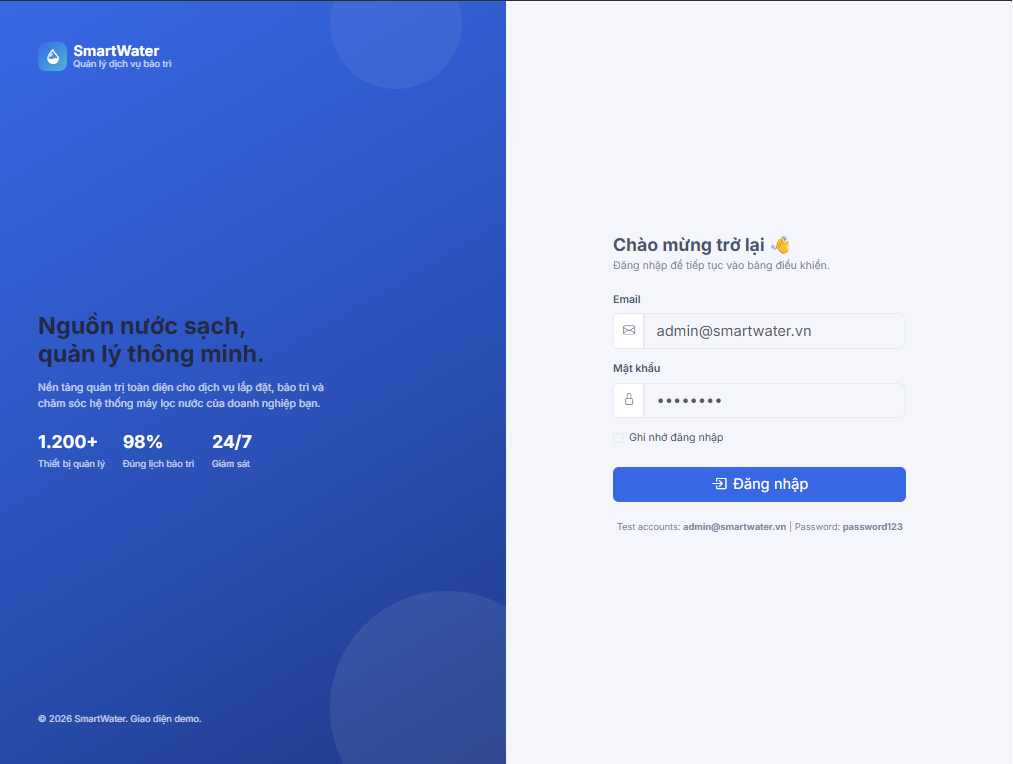
\includegraphics[width=0.90\linewidth]{include/web-UI/smartwater-admin-login.png}
    \caption{Giao diện đăng nhập SmartWater Admin}
    \label{fig:week7-admin-login}
\end{figure}

\begin{figure}[H]
    \centering
    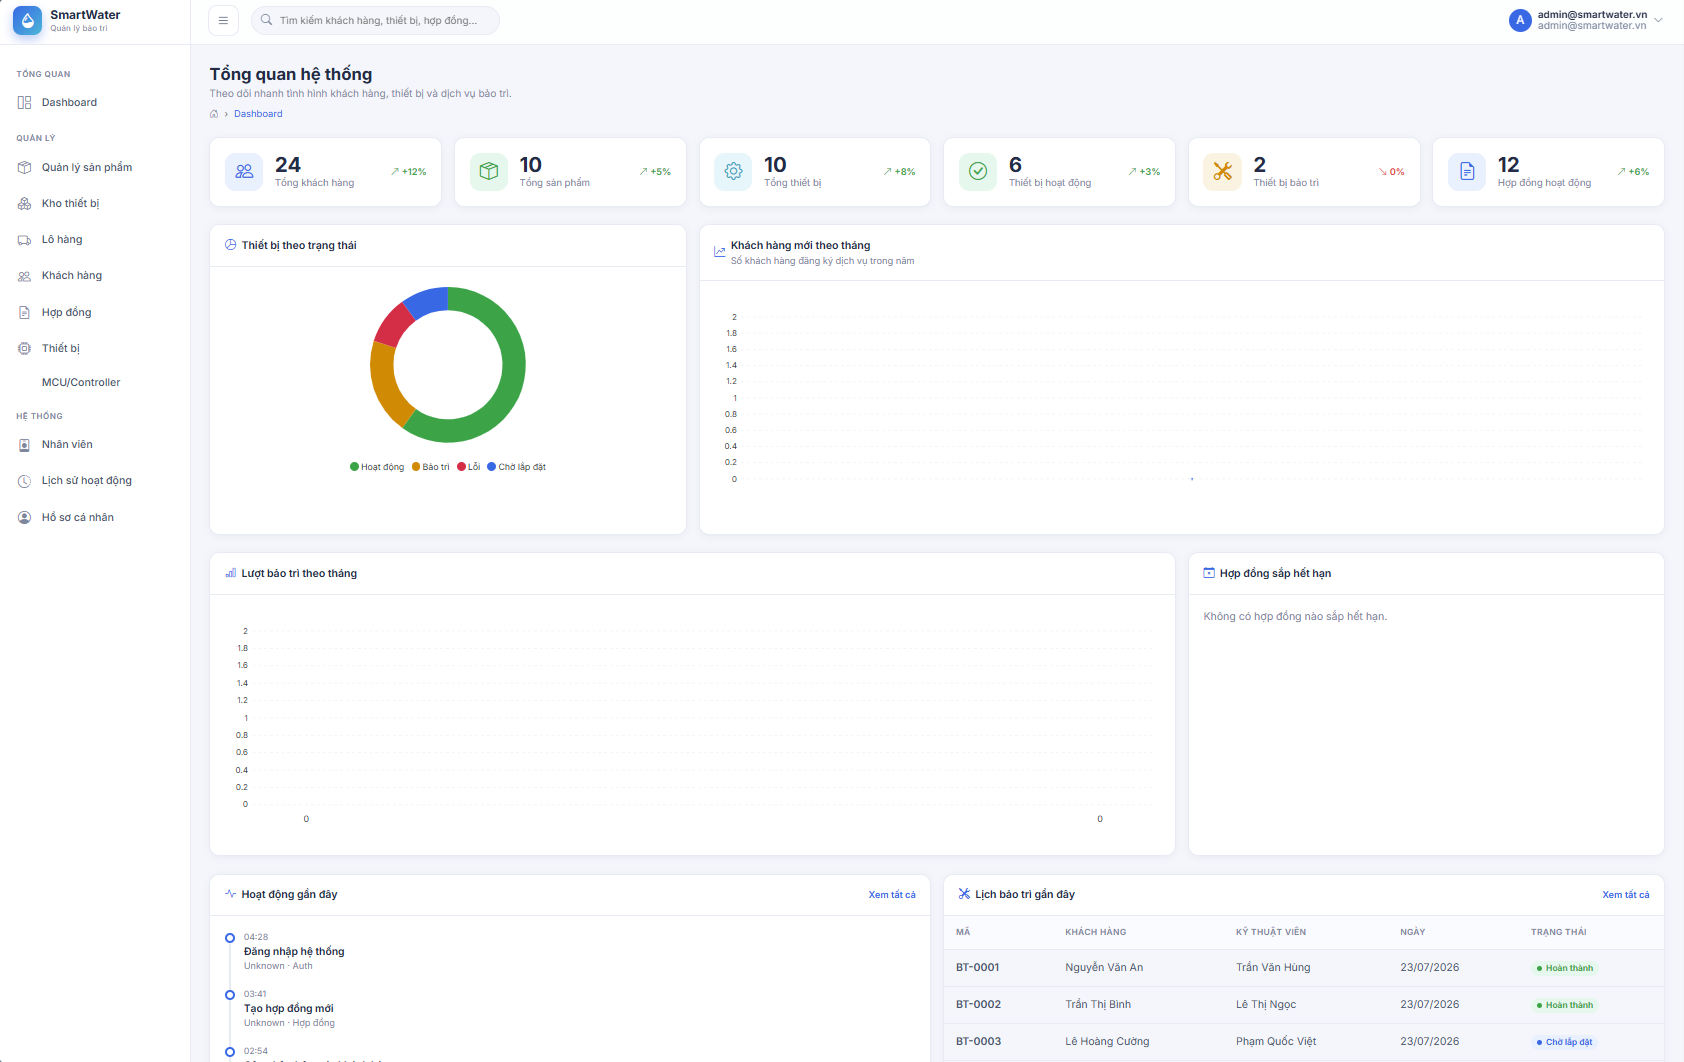
\includegraphics[width=0.95\linewidth]{include/web-UI/smartwater-admin-main.png}
    \caption{Dashboard tổng quan SmartWater Admin}
    \label{fig:week7-admin-dashboard}
\end{figure}

\subsubsubsection*{6.2.8.3 Quản lý danh mục, sản phẩm, kho và lô hàng}

Module sản phẩm là dữ liệu nền cho thiết bị và kho. Mỗi sản phẩm thuộc một danh mục; tồn kho được quản lý theo sản phẩm, còn lô hàng và chi tiết lô hàng hỗ trợ truy vết nguồn nhập. Các màn hình danh sách cung cấp khả năng xem, tìm kiếm và thao tác quản trị theo route của từng module.

\begin{figure}[H]
    \centering
    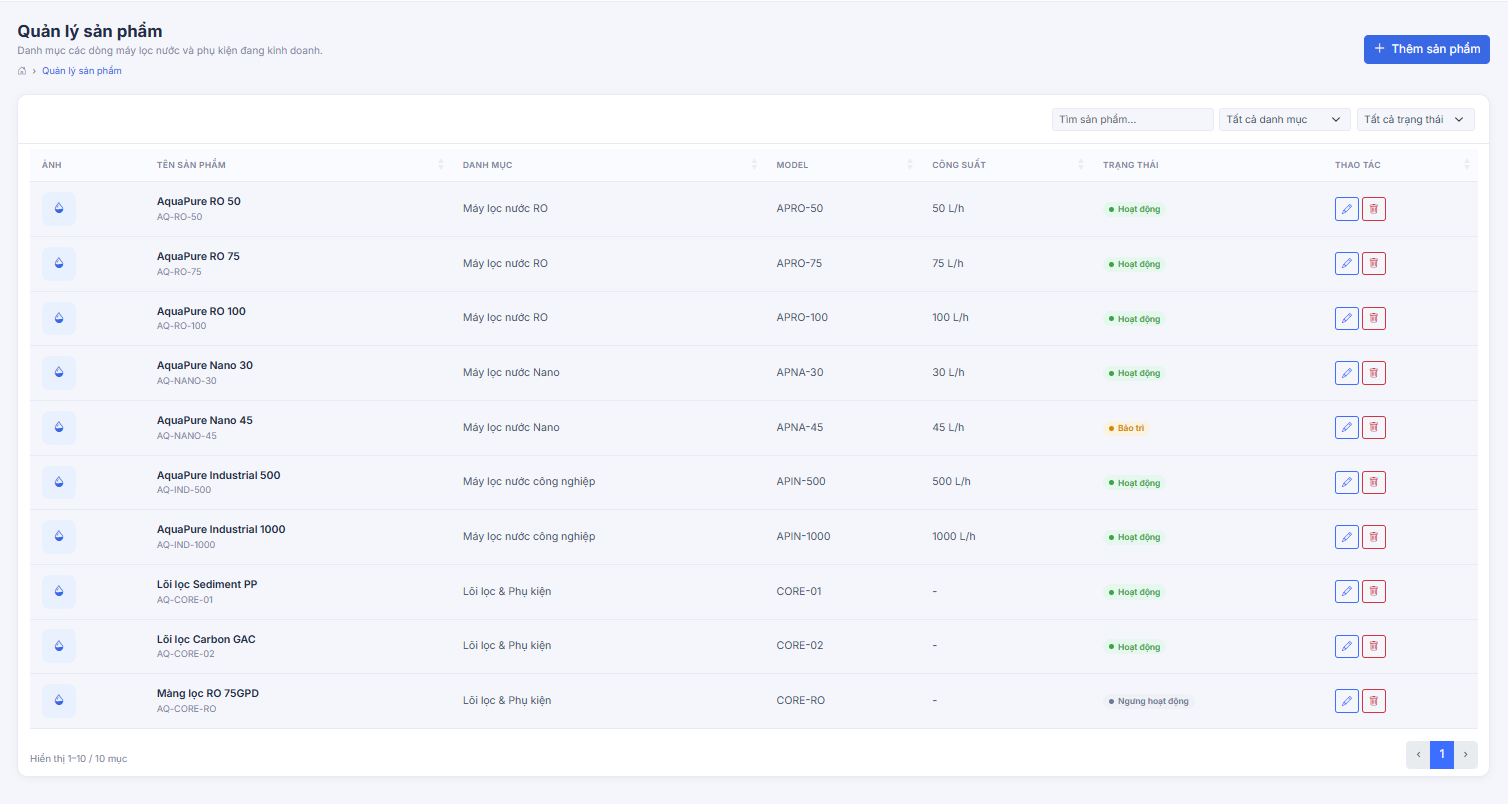
\includegraphics[width=0.90\linewidth]{include/web-UI/smartwater-admin-product.png}
    \caption{Giao diện quản lý sản phẩm}
    \label{fig:week7-admin-product}
\end{figure}

\begin{figure}[H]
    \centering
    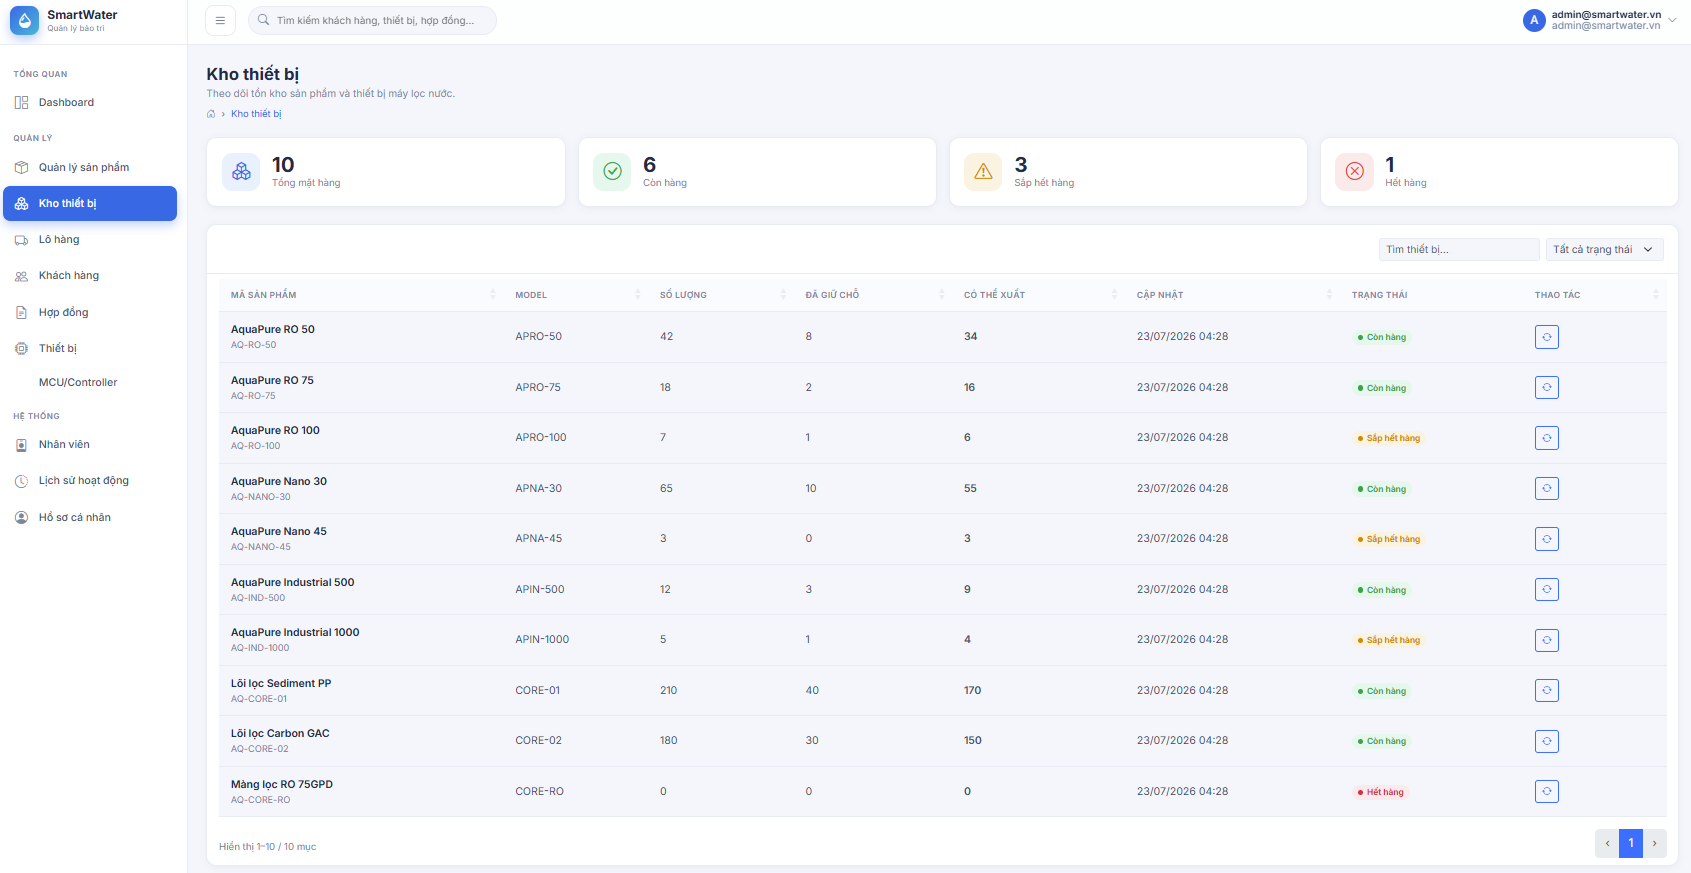
\includegraphics[width=0.90\linewidth]{include/web-UI/smartwater-admin-inventory.png}
    \caption{Giao diện quản lý tồn kho}
    \label{fig:week7-admin-inventory}
\end{figure}

\begin{figure}[H]
    \centering
    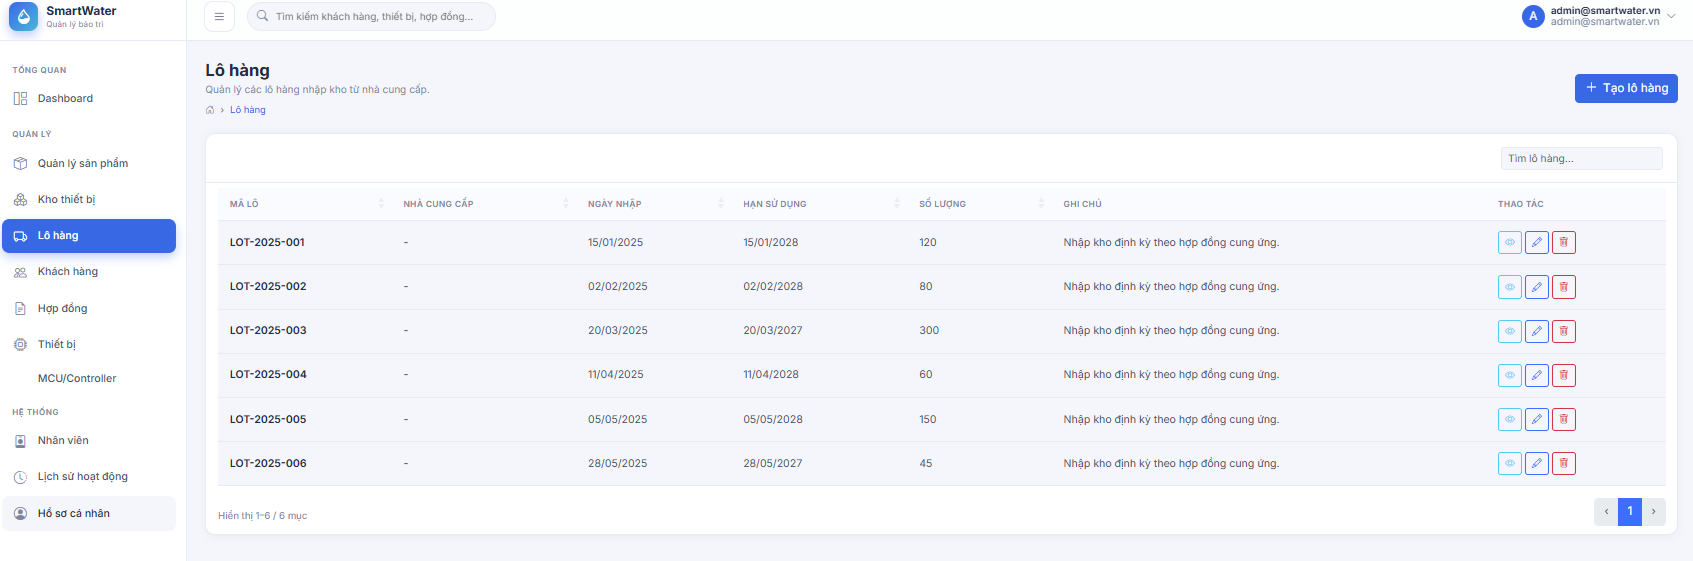
\includegraphics[width=0.90\linewidth]{include/web-UI/smartwater-admin-batch.png}
    \caption{Giao diện quản lý lô hàng}
    \label{fig:week7-admin-batch}
\end{figure}

\subsubsubsection*{6.2.8.4 Quản lý khách hàng và hợp đồng}

Nhóm chức năng khách hàng và hợp đồng thể hiện dữ liệu nghiệp vụ xuyên suốt quá trình lắp đặt và vận hành máy lọc nước. Một khách hàng có thể có nhiều hợp đồng; thiết bị được gắn với khách hàng và hợp đồng phù hợp để hỗ trợ truy vết khi xem thông tin vận hành hoặc lịch sử bảo trì.

\begin{figure}[H]
    \centering
    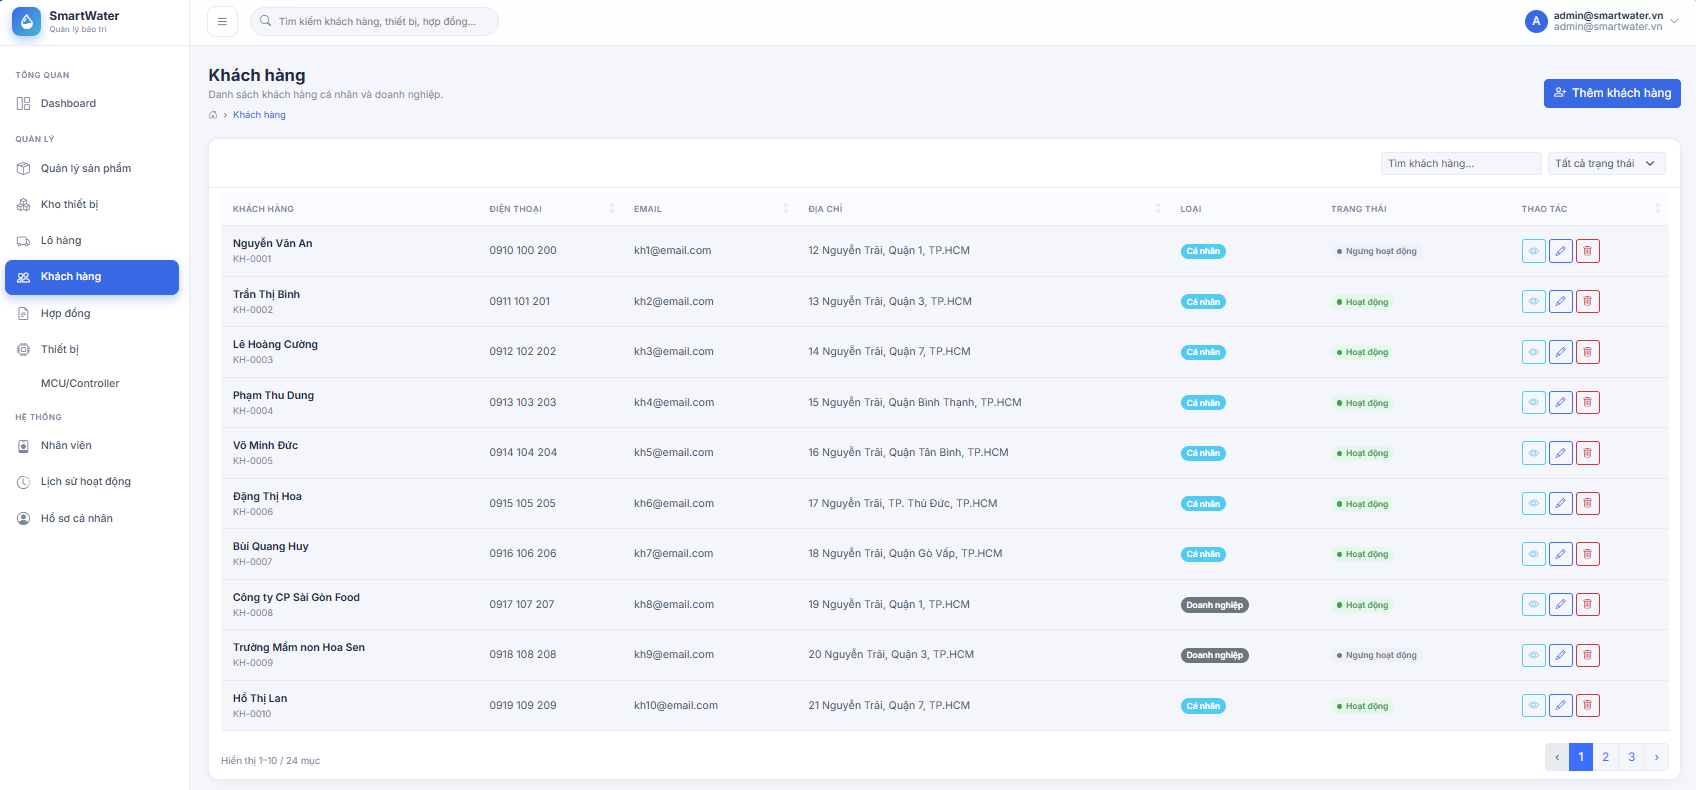
\includegraphics[width=0.90\linewidth]{include/web-UI/smartwater-admin-customer.png}
    \caption{Danh sách khách hàng trong SmartWater Admin}
    \label{fig:week7-admin-customer}
\end{figure}

\begin{figure}[H]
    \centering
    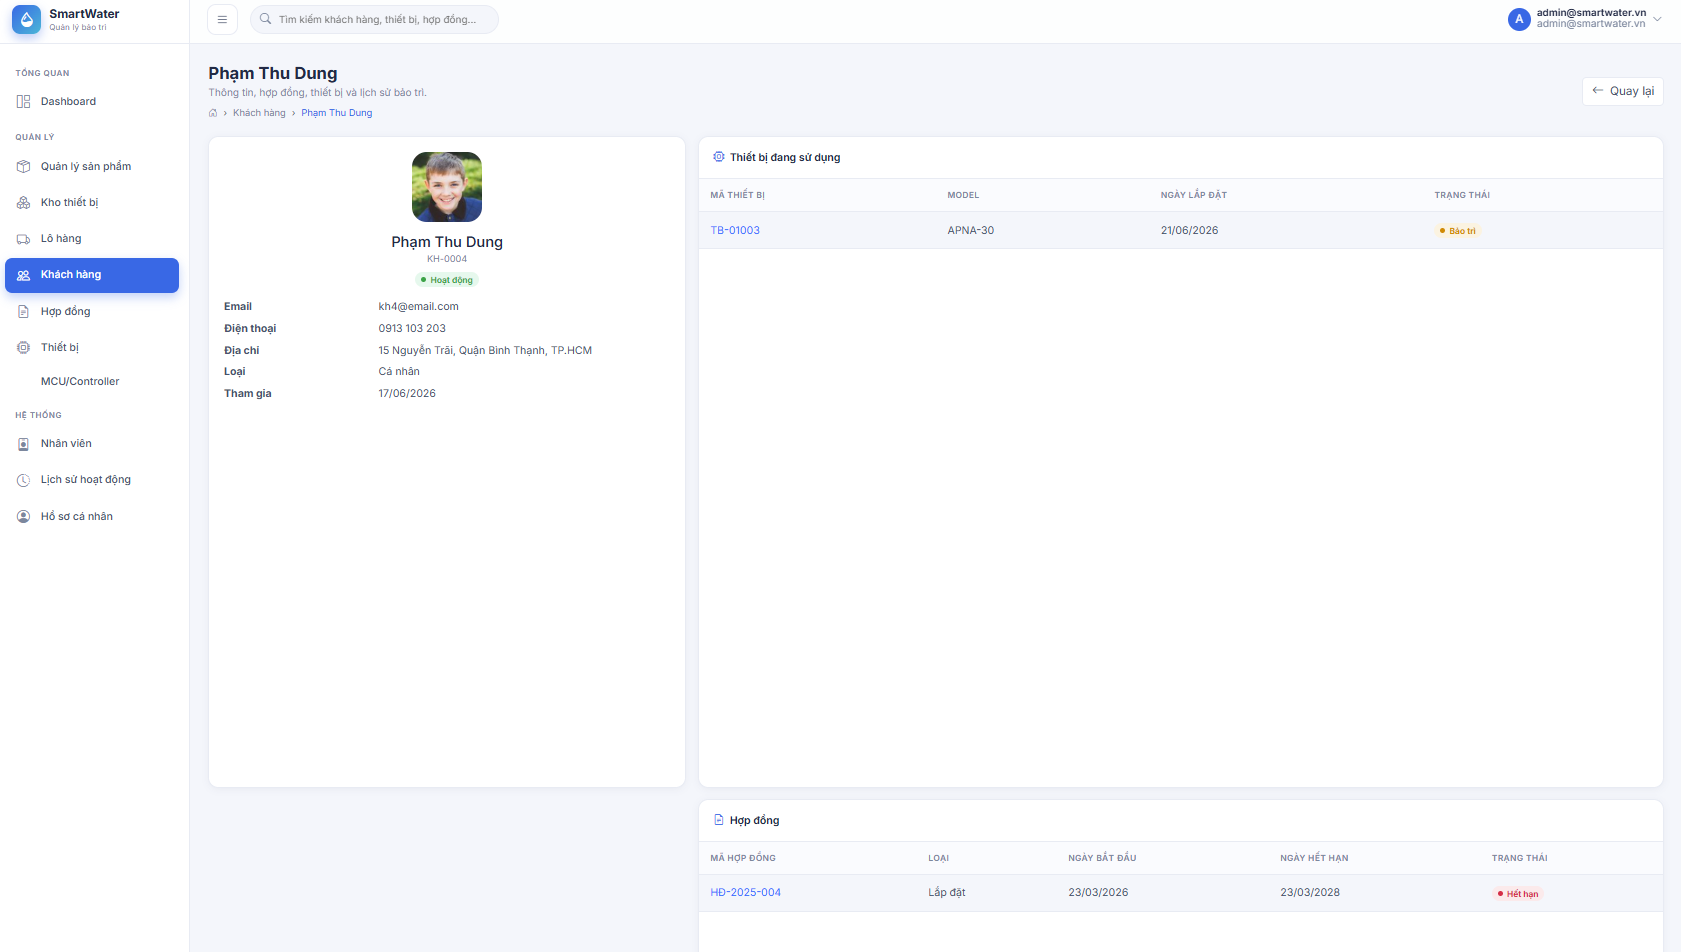
\includegraphics[width=0.90\linewidth]{include/web-UI/smartwater-admin-customer-profile.png}
    \caption{Hồ sơ và thông tin liên quan của khách hàng}
    \label{fig:week7-admin-customer-profile}
\end{figure}

\begin{figure}[H]
    \centering
    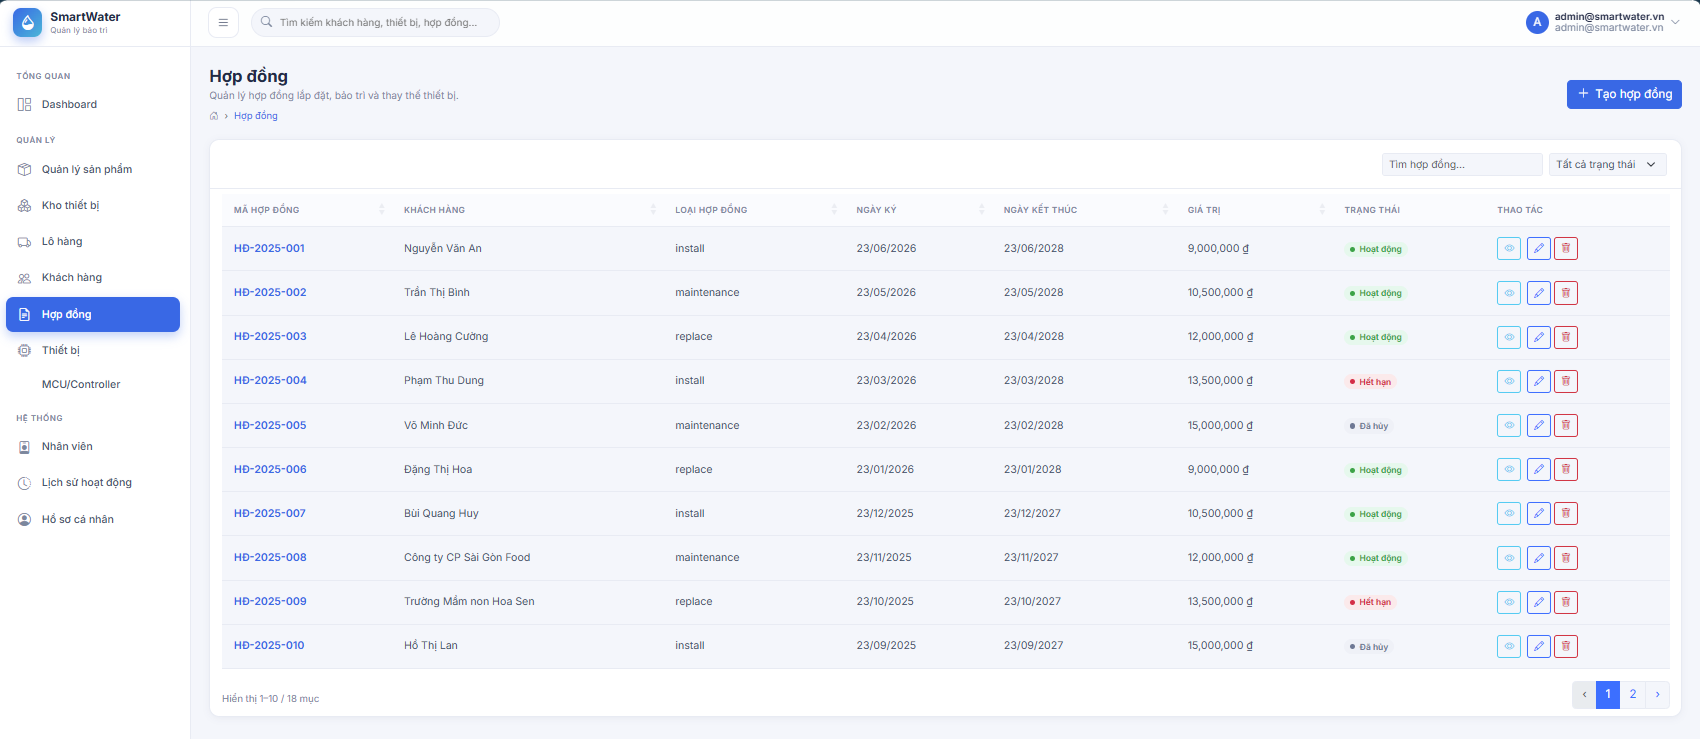
\includegraphics[width=0.90\linewidth]{include/web-UI/smartwater-admin-contract.png}
    \caption{Giao diện quản lý hợp đồng}
    \label{fig:week7-admin-contract}
\end{figure}

\subsubsubsection*{6.2.8.5 Quản lý thiết bị, MCU và telemetry}

Module thiết bị liên kết Product, Customer, Contract và MCU. MCU được nhận diện bằng \texttt{mcu\_id} dạng chuỗi; Device lưu \texttt{mcu\_id} để gắn một MCU vào thiết bị. Khi xem chi tiết thiết bị, dữ liệu telemetry được đọc theo MCU để phục vụ theo dõi TDS và trạng thái cảnh báo.

\begin{figure}[H]
    \centering
    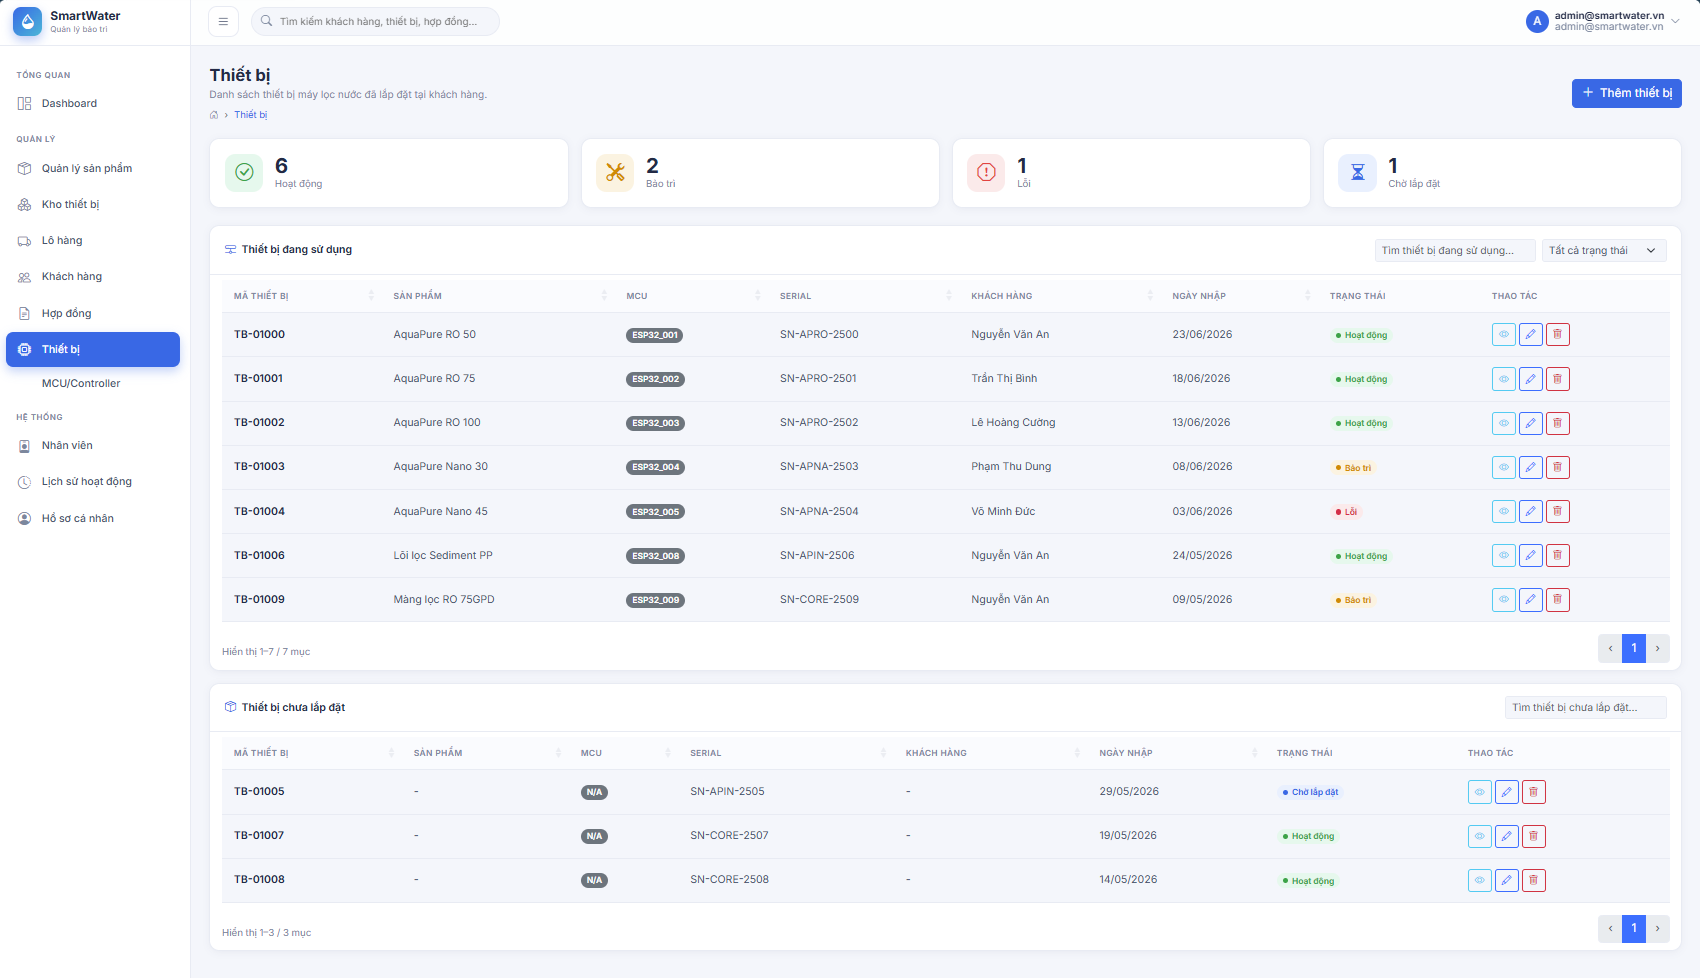
\includegraphics[width=0.90\linewidth]{include/web-UI/smartwater-admin-device.png}
    \caption{Giao diện quản lý thiết bị}
    \label{fig:week7-admin-device}
\end{figure}

\begin{figure}[H]
    \centering
    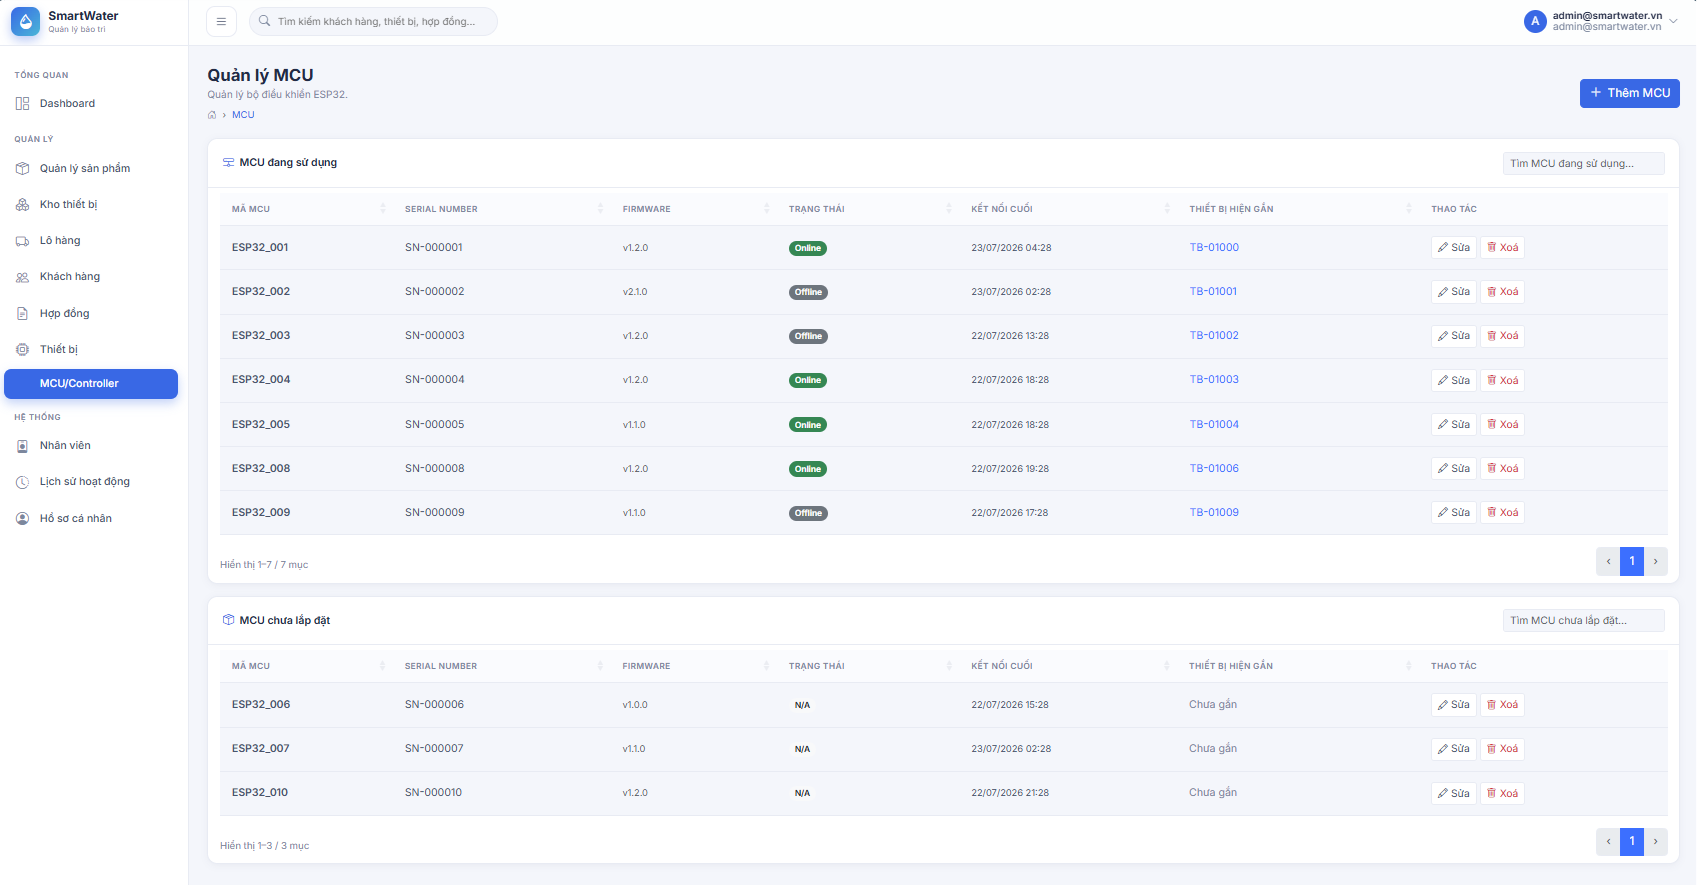
\includegraphics[width=0.90\linewidth]{include/web-UI/smartwater-admin-mcu.png}
    \caption{Giao diện quản lý MCU}
    \label{fig:week7-admin-mcu}
\end{figure}

\begin{figure}[H]
    \centering
    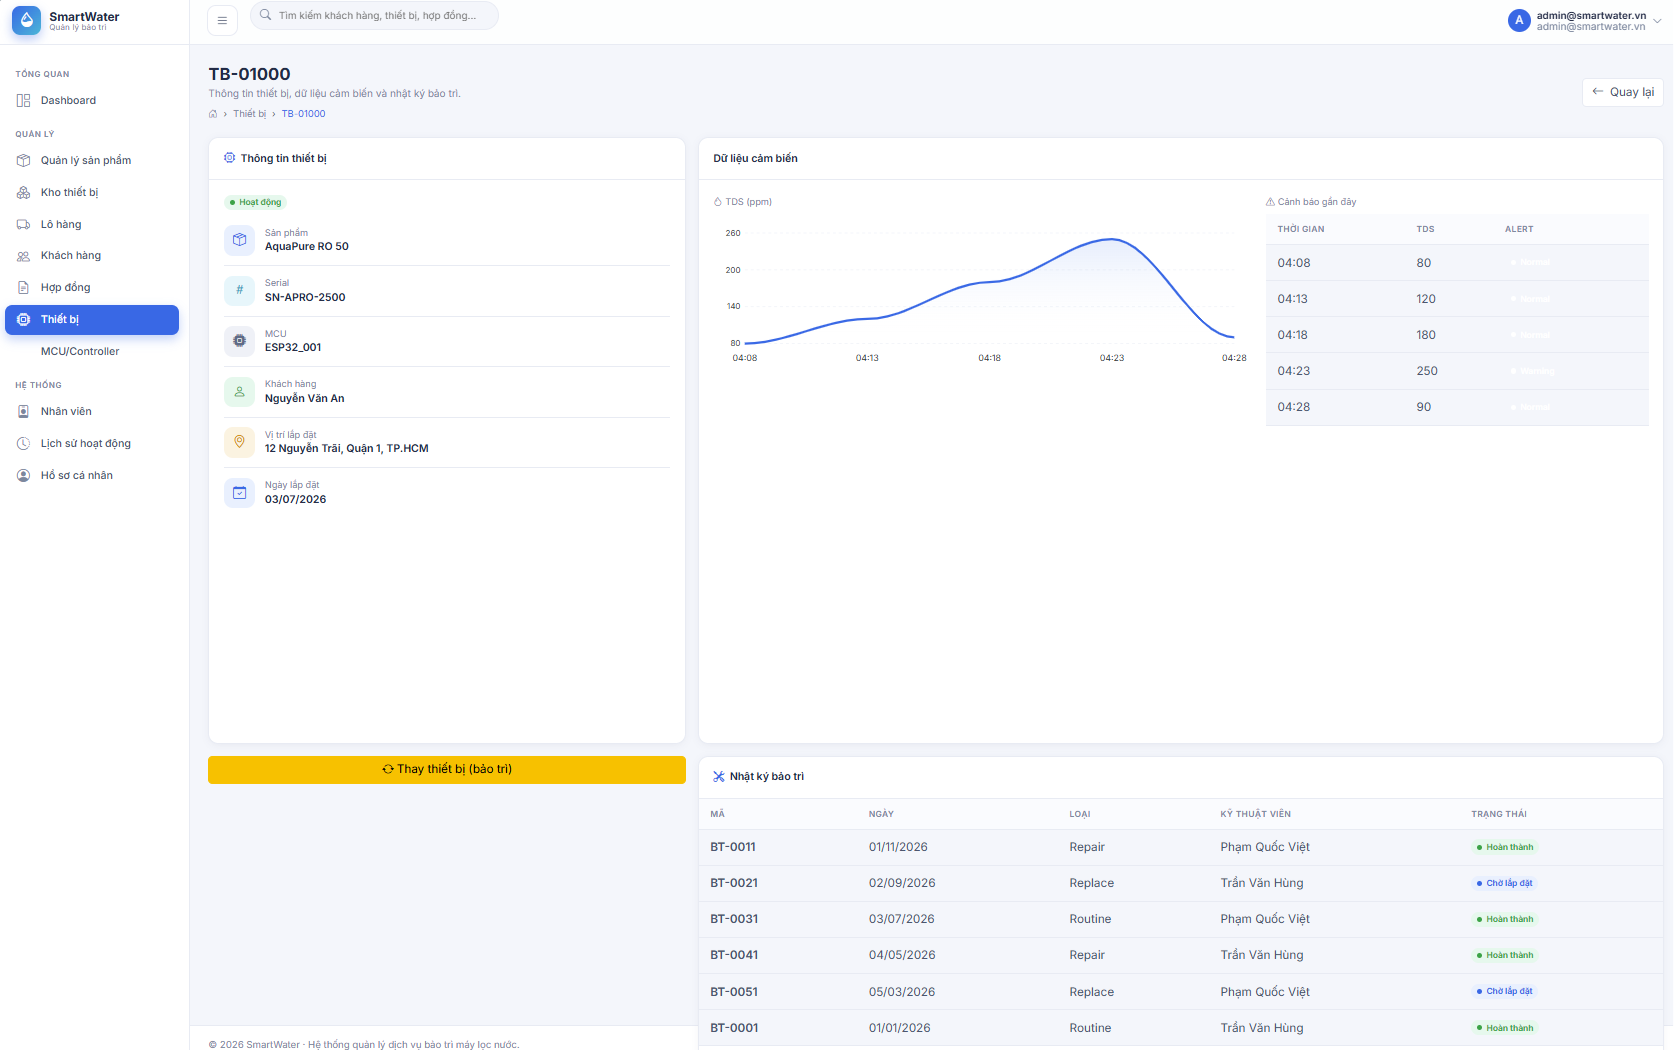
\includegraphics[width=0.90\linewidth]{include/web-UI/smartwater-admin-device-telemetry.png}
    \caption{Telemetry trong màn hình chi tiết thiết bị}
    \label{fig:week7-admin-device-telemetry}
\end{figure}

\subsubsubsection*{6.2.8.6 Nhân viên, hoạt động và hồ sơ người dùng}

Các module nhân viên, lịch sử hoạt động và hồ sơ giúp hỗ trợ vận hành hệ thống. Nhân viên được gắn với vai trò để phân quyền; hoạt động được lưu trong \texttt{activity\_logs}; màn hình hồ sơ cho phép người dùng xem và cập nhật thông tin cá nhân.

\begin{figure}[H]
    \centering
    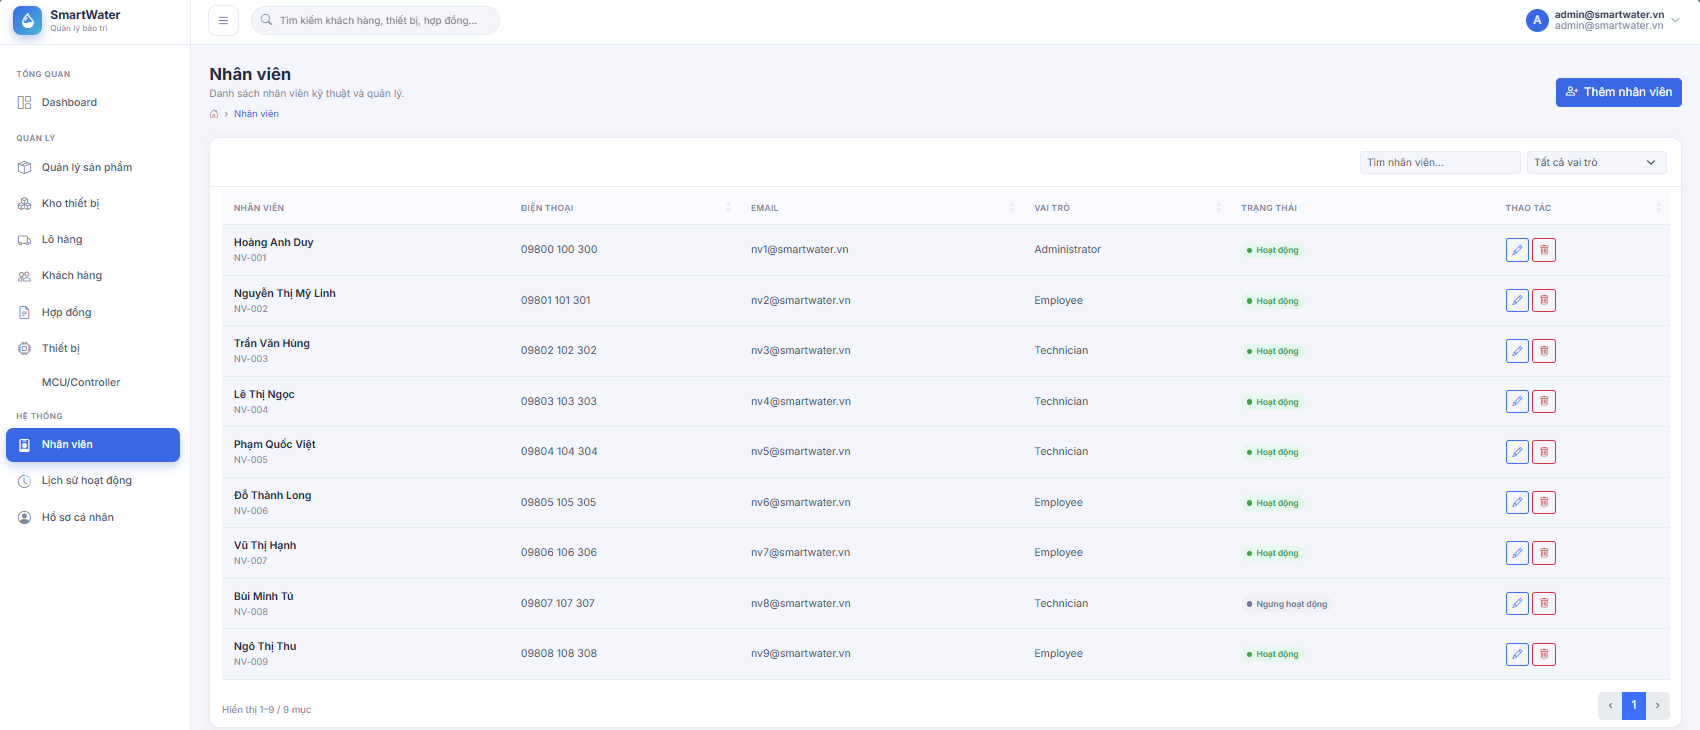
\includegraphics[width=0.90\linewidth]{include/web-UI/smartwater-admin-employee.png}
    \caption{Giao diện quản lý nhân viên}
    \label{fig:week7-admin-employee}
\end{figure}

\begin{figure}[H]
    \centering
    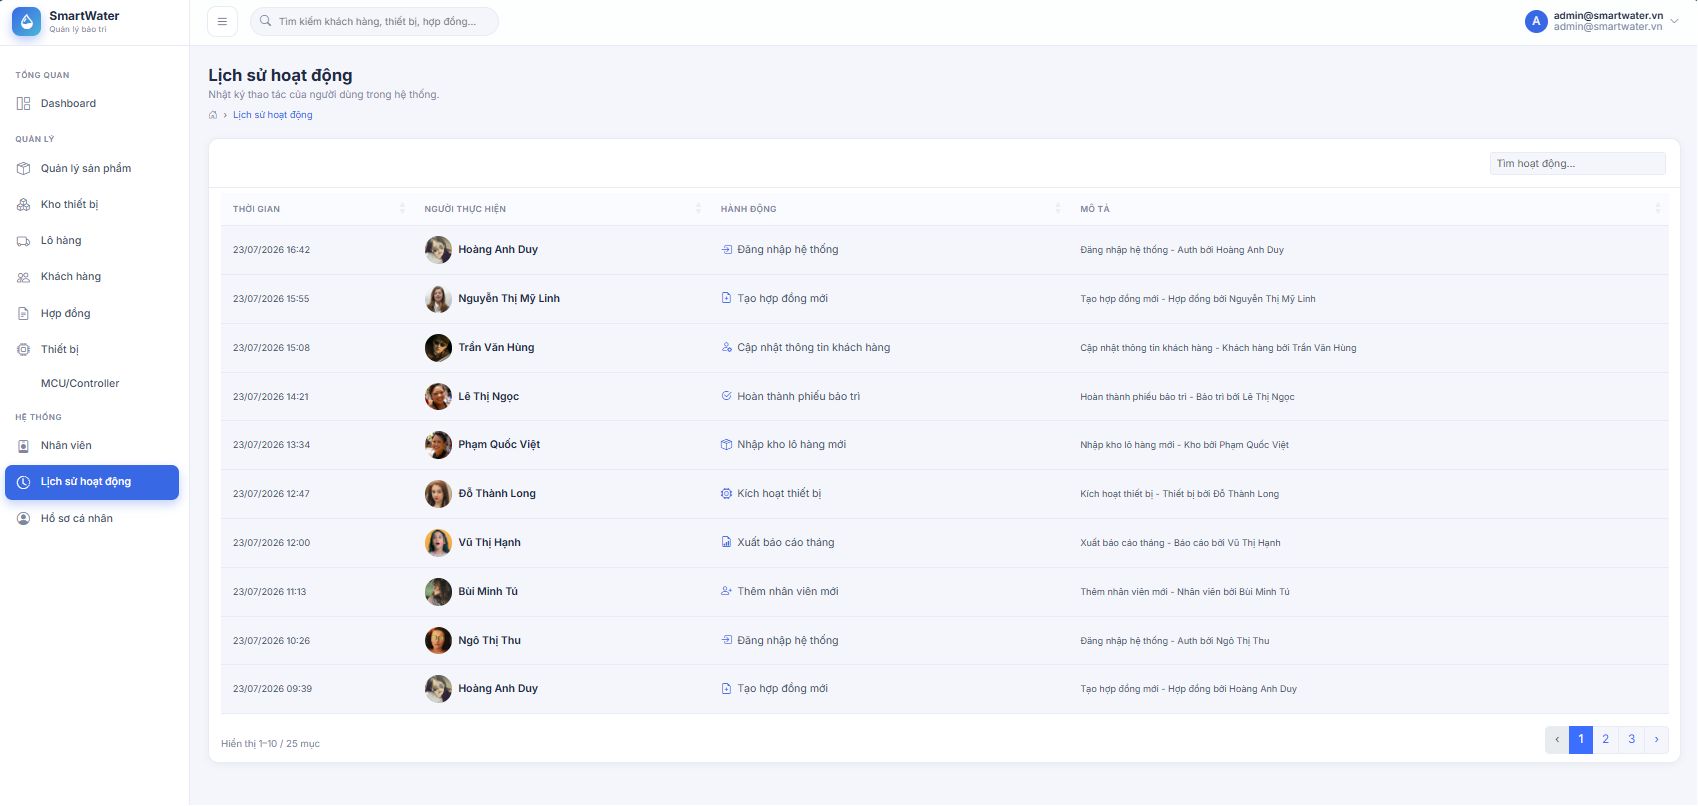
\includegraphics[width=0.90\linewidth]{include/web-UI/smartwater-admin-history.png}
    \caption{Giao diện lịch sử hoạt động}
    \label{fig:week7-admin-history}
\end{figure}

\begin{figure}[H]
    \centering
    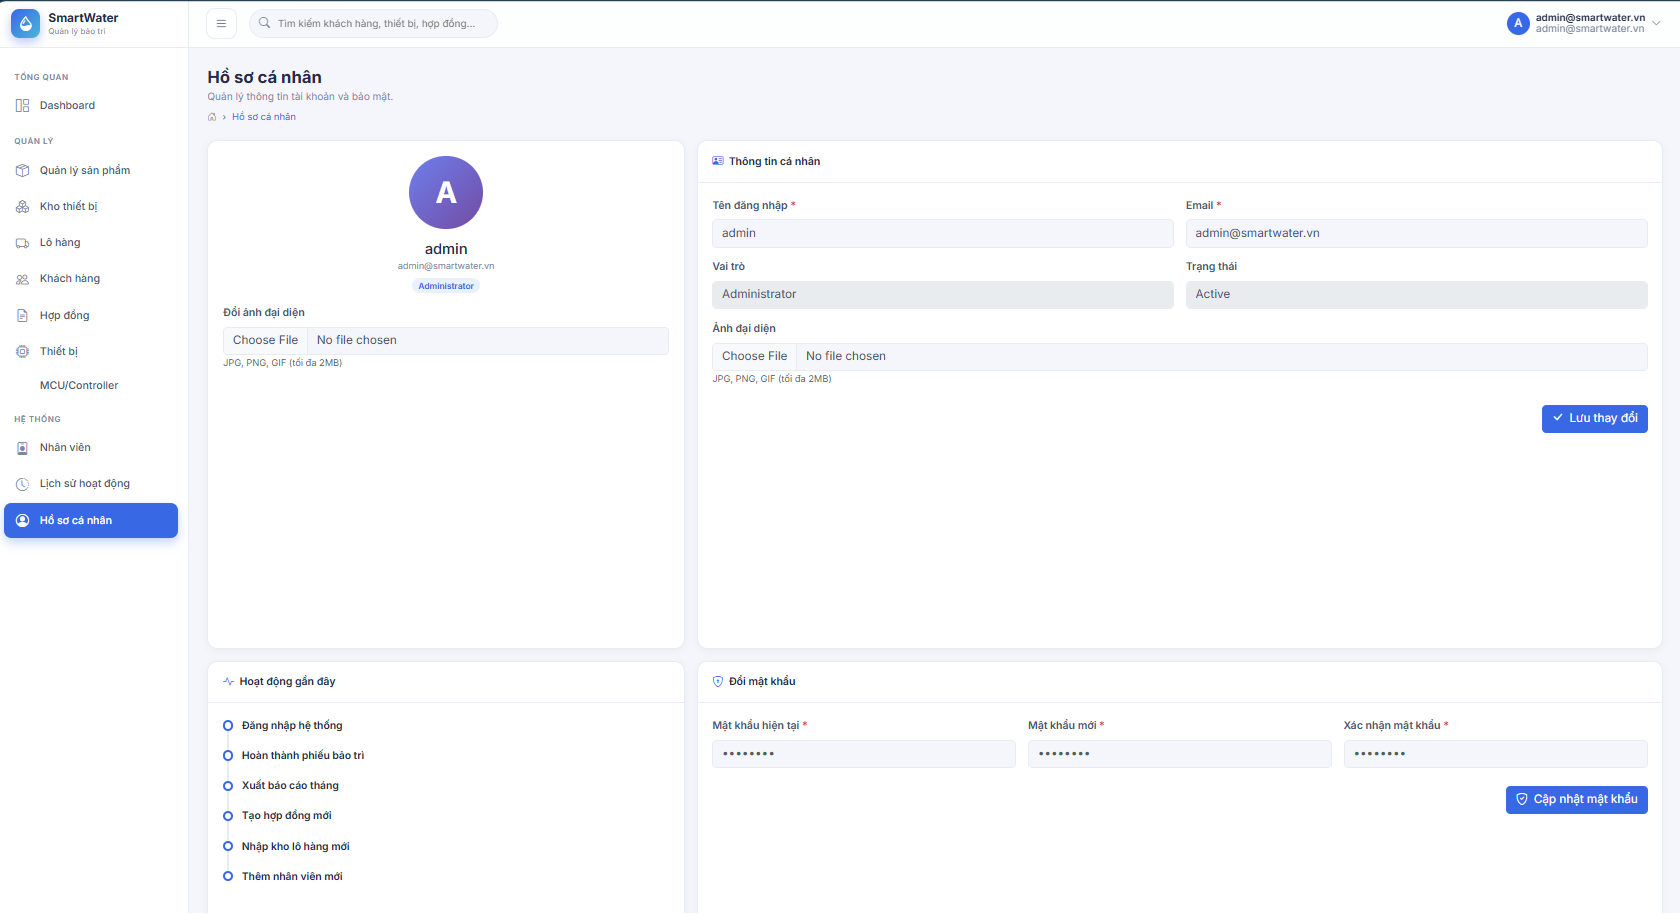
\includegraphics[width=0.90\linewidth]{include/web-UI/smartwater-admin-profile.png}
    \caption{Giao diện hồ sơ người dùng}
    \label{fig:week7-admin-profile}
\end{figure}

\subsubsubsection*{6.3.1 Kết quả xây dựng SmartWater Admin}

Sinh viên kiểm tra luồng điều hướng từ đăng nhập đến các module quản trị, đồng thời đối chiếu dữ liệu hiển thị với các route, controller, service và model của SmartWater Admin. Dashboard có source truy vấn KPI, phân bố thiết bị, khách hàng theo tháng, bảo trì, hoạt động gần đây và hợp đồng sắp hết hạn. Các module sản phẩm, kho, khách hàng, hợp đồng, thiết bị, MCU, nhân viên và hồ sơ đều có màn hình giao diện tương ứng.

Kết quả đạt được:

\begin{itemize}
    \item Hoàn thiện giao diện đăng nhập và dashboard tổng quan cho SmartWater Admin.
    \item Tổ chức các chức năng quản trị theo từng module nghiệp vụ rõ ràng.
    \item Hiển thị được chuỗi dữ liệu Customer--Contract--Product--Device--MCU và telemetry liên quan.
    \item Cung cấp giao diện theo dõi telemetry tại chi tiết thiết bị; dữ liệu TDS được khai thác từ bảng telemetry dùng chung.
    \item Bổ sung các màn hình hỗ trợ vận hành gồm tồn kho, lô hàng, nhân viên, lịch sử và hồ sơ.
\end{itemize}

Phần giao diện quản trị được gộp vào Week 6 để hoàn thiện luồng từ thu nhận telemetry đến khai thác dữ liệu nghiệp vụ. Các phần cần tiếp tục hoàn thiện gồm kiểm thử runtime đầy đủ cho từng module và thay thế xu hướng KPI cố định bằng dữ liệu so sánh thực tế.


\subsubsection*{6.3 Kiểm thử và kết quả đạt được}

Sinh viên thực hiện kiểm thử toàn bộ luồng bằng firmware mô phỏng. ESP32 publish telemetry lên HiveMQ, Device Monitor subscribe bản tin, gọi API, làm phẳng payload lồng, chuẩn hóa dữ liệu và ghi vào MySQL. Sau đó dữ liệu được kiểm tra trên danh sách MCU, bảng telemetry đã lọc và biểu đồ TDS.

Hình \ref{fig:week6-hivemq-message} là bằng chứng ESP32 simulator đã publish thành công các bản tin lên topic \texttt{devices/telemetry}. HiveMQ Web Client nhận ba message có \texttt{mcu\_id} \texttt{ESP32\_001} và dữ liệu TDS trong object \texttt{telemetry}.

\begin{figure}[H]
    \centering
    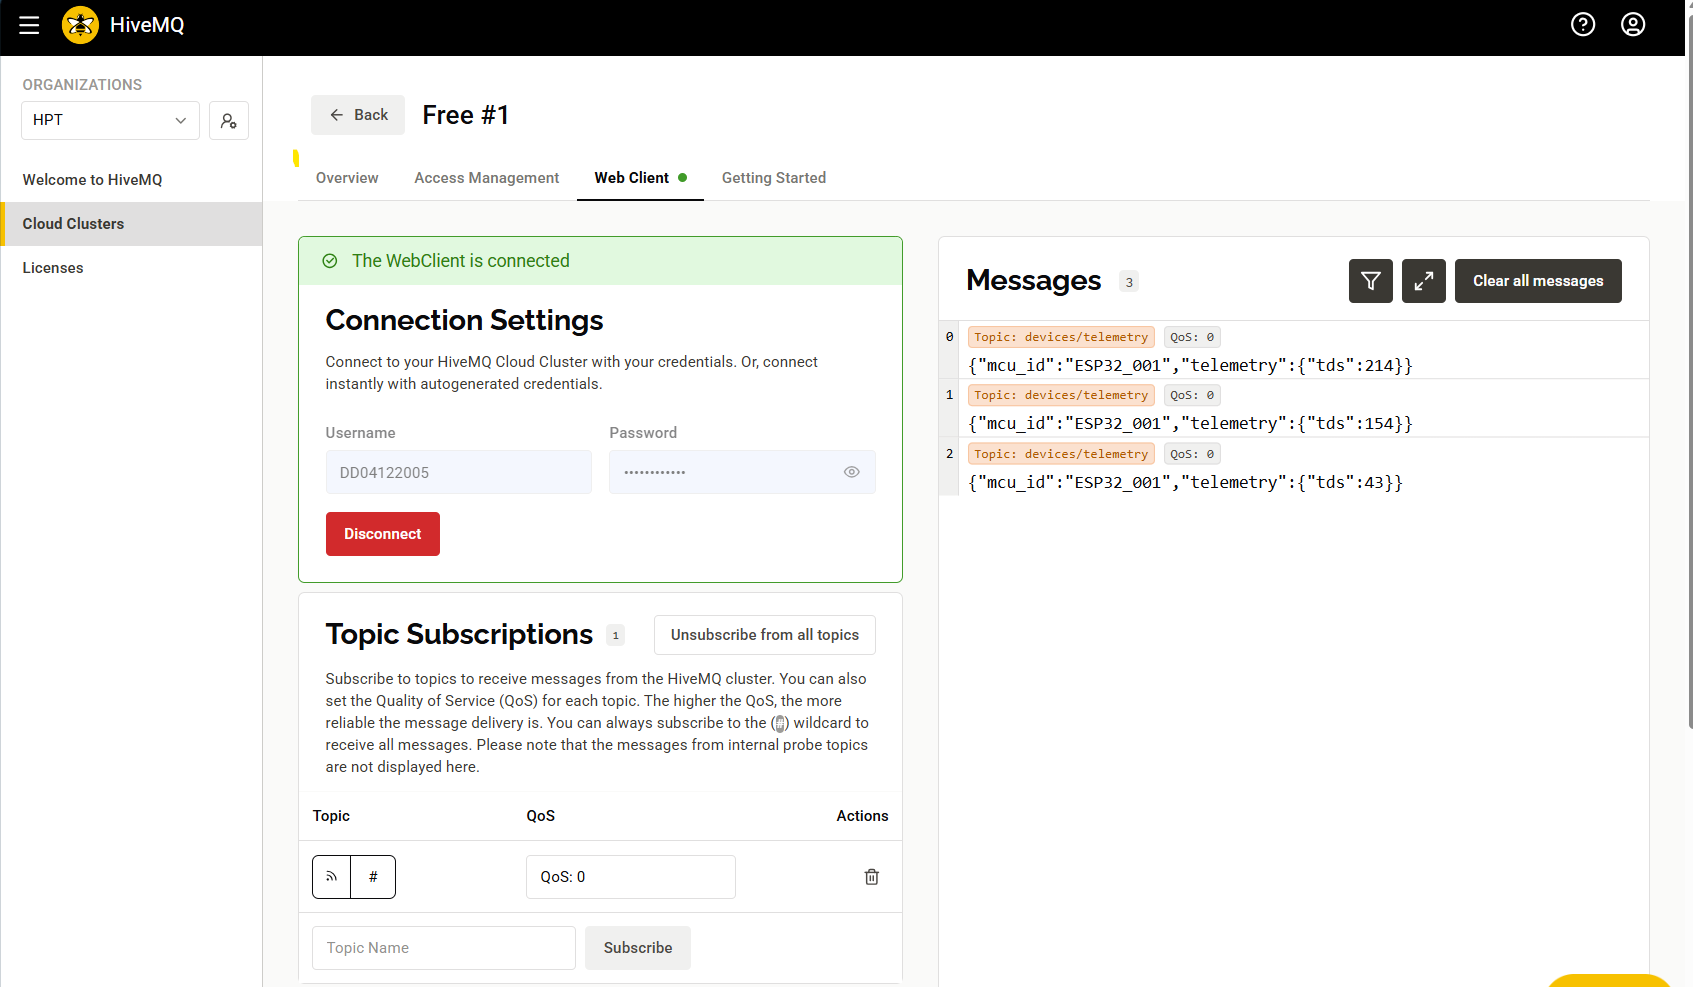
\includegraphics[width=0.95\linewidth]{include/image/hivemq-message.png}
    \caption{HiveMQ Web Client nhận telemetry được ESP32 simulator publish thành công}
    \label{fig:week6-hivemq-message}
\end{figure}

Kết quả đạt được:

\begin{itemize}
    \item Device Monitor kết nối và subscribe được HiveMQ Cloud.
    \item Payload được parse và chuẩn hóa thống nhất.
    \item Telemetry được lưu đúng bảng với \texttt{mcu\_id} dạng chuỗi và timestamp UTC do Device Monitor tạo.
    \item Telemetry Live hiển thị MCU không trùng, bảng dữ liệu theo MCU và biểu đồ TDS theo thời gian.
    \item Dữ liệu mẫu xác nhận chuỗi Customer--Contract--Product--Device--MCU--Telemetry có thể được tạo bằng \texttt{ConnectedTelemetryDemoSeeder}.
    \item Luồng ESP32 $\rightarrow$ HiveMQ $\rightarrow$ Device Monitor $\rightarrow$ MySQL $\rightarrow$ Dashboard hoạt động thống nhất.
\end{itemize}

Kết quả tuần 6 hoàn thiện nền tảng thu nhận và giám sát telemetry của SmartWater, làm cơ sở cho các chức năng quản lý thiết bị, cảnh báo và bảo trì ở những giai đoạn tiếp theo.
